%%%%%%%%%%%%%%%%%%%%%%% file template.tex %%%%%%%%%%%%%%%%%%%%%%%%%
%
% This is a general template file for the LaTeX package SVJour3
% for Springer journals.          Springer Heidelberg 2010/09/16
%
% Copy it to a new file with a new name and use it as the basis
% for your article. Delete % signs as needed.
%
% This template includes a few options for different layouts and
% content for various journals. Please consult a previous issue of
% your journal as needed.
%
%%%%%%%%%%%%%%%%%%%%%%%%%%%%%%%%%%%%%%%%%%%%%%%%%%%%%%%%%%%%%%%%%%%
%
% First comes an example EPS file -- just ignore it and
% proceed on the \documentclass line
% your LaTeX will extract the file if required
\begin{filecontents*}{example.eps}
%!PS-Adobe-3.0 EPSF-3.0
%%BoundingBox: 19 19 221 221
%%CreationDate: Mon Sep 29 1997
%%Creator: programmed by hand (JK)
%%EndComments
gsave
newpath
  20 20 moveto
  20 220 lineto
  220 220 lineto
  220 20 lineto
closepath
2 setlinewidth
gsave
  .4 setgray fill
grestore
stroke
grestore
\end{filecontents*}
%
\RequirePackage{fix-cm}

\documentclass[smallextended]{svjour3}

\smartqed  % flush right qed marks, e.g. at end of proof
%
\usepackage{graphicx}

\usepackage[authoryear]{natbib}  %% The order is important

\usepackage[resetlabels]{multibib}
\newcites{inappendix}{Supplementary References}

% \usepackage{alifeconf}

\usepackage{hyperref}

\usepackage{subcaption}

\usepackage{hhline}

\usepackage{amsmath}

\usepackage{rotating}

\usepackage{bibspacing}
\setlength{\bibsep}{0pt plus 0.3ex}

\usepackage{geometry}

\ifdefined\mydraft
\mydraft
\fi

% \usepackage[
%   %subtle
%   moderate
% ]{savetrees}

\graphicspath{{img/}}

% *****************
%  Requirements:
% *****************
%
% - All pages sized consistently at 8.5 x 11 inches (US letter size).
% - PDF length <= 8 pages for full papers, <=2 pages for extended
%    abstracts.
% - Abstract length <= 250 words.
% - No visible crop marks.
% - Images at no greater than 300 dpi, scaled at 100%.
% - Embedded open type fonts only.
% - All layers flattened.
% - No attachments.
% - All desired links active in the files.

% Note that the PDF file must not exceed 5 MB if it is to be indexed
% by Google Scholar. Additional information about Google Scholar
% can be found here:
% http://www.google.com/intl/en/scholar/inclusion.html.


% If your system does not generate letter format documents by default,
% you can use the following workflow:
% latex example
% bibtex example
% latex example ; latex example
% dvips -o example.ps -t letterSize example.dvi
% ps2pdf example.ps example.pdf


% For pdflatex users:
% The alifeconf style file loads the "graphicx" package, and
% this may lead some users of pdflatex to experience problems.
% These can be fixed by editing the alifeconf.sty file to specify:
% \usepackage[pdftex]{graphicx}
%   instead of
% \usepackage{graphicx}.
% The PDF output generated by pdflatex should match the required
% specifications and obviously the dvips and ps2pdf steps become
% unnecessary.


% Note:  Some laser printers have a serious problem printing TeX
% output. The use of ps type I fonts should avoid this problem.


\title{Matchmaker, Matchmaker, Make Me a Match: Geometric, Variational, and Evolutionary Implications of Criteria for Tag Affinity}
\titlerunning{Matchmaker, Matchmaker, Make Me a Match}
\author{
    Matthew Andres Moreno
	  \and Alexander Lalejini
    \and Charles Ofria \\
}

\authorrunning{Moreno et al.} % if too long for running head

\institute{%
  M. A. Moreno \at
  BEACON Center for the Study of Evolution in Action \\
  Department of Computer Science and Engineering \\
  Program in Ecology, Evolutionary Biology, and Behavior \\
  Michigan State University, East Lansing, MI \\
  \email{mmore500@msu.edu}
\and
  A. Lalejini \at
  University of Michigan, Ann Arbor, MI \\
\and
  C. Ofria \at
  BEACON Center for the Study of Evolution in Action \\
  Department of Computer Science and Engineering \\
  Program in Ecology, Evolutionary Biology, and Behavior \\
  Michigan State University, East Lansing, MI \\
}

\date{Received: date / Accepted: date}

% For several authors from the same institution use the same number to
% refer to one address.
%
% If the names do not fit well on one line use
%         Author 1, Author 2 ... \\ {\Large\bf Author n} ...\\ ...
%
% If the title and author information do not fit in the area
% allocated, place \setlength\titlebox{<new height>} after the
% \documentclass line where <new height> is 2.25in



\begin{document}
\maketitle

\begin{abstract}

Genetic programming and artificial life systems commonly employ tag-matching schemes to determine interactions between model components.
%Criteria to determine affinity between tags %TODO
However, the implications of criteria used to determine affinity between tags with respect to constraints on emergent connectivity, canalization of changes to connectivity under mutation, and evolutionary dynamics have not been considered.
We highlight differences between tag-matching criteria with respect to geometric constraint and variation generated under mutation. 
We find that tag-matching criteria can influence the rate of adaptive evolution and the quality of evolved solutions.
Better understanding of the geometric, variational, and evolutionary properties of tag-matching criteria will facilitate more effective incorporation of tag matching into genetic programming and artificial life systems.
By showing that tag-matching criteria influence connectivity patterns and evolutionary dynamics, our findings also raise fundamental questions about the properties of tag-matching systems in nature.

\keywords{Genetic Programming \and Event-driven Genetic Programming \and Tag-based Referencing \and Module-based Genetic Programming \and Artificial Gene Regulatory Networks}
% \PACS{PACS code1 \and PACS code2 \and more}
% \subclass{MSC code1 \and MSC code2 \and more}

\end{abstract}


\section{Introduction}

TODO \citep{taylor2016open}

\subsection{What is a tag?}

At a broad level, tags are labels that can be used to refer to labelees (the
tagged thing).

\subsubsection{Examples of tags}

\begin{itemize}
  \item Human culture (probably don't want to draw too many examples from this category)
    \begin{itemize}
      \item We name our offspring, which is useful for later referring to them.
            Names are often repeated across individuals (e.g., we'll be seeing an
            uptick in `Arya's post-GoT). Context + multi-level naming (first, middle,
            last in 20th century American culture) is important for resolving collisions.
    \end{itemize}
  \item Software development
    \begin{itemize}
      \item In software development, we label and refer to lots of things! In this
            domain, tags are precise: after labeling (tagging) something, subsequent
            referrals to those labeled things must be \textit{exact}. Inexactness
            in a reference typically results in syntactic errors.
      \item Common uses: labeling and specifying locations in memory, custom data
            structures (e.g., structs, classes, etc), functions, libraries/modules,
            language constants/built-ins, program entry points, locations in an
            instruction sequence (e.g., function names, looping, conditionals etc).
    \end{itemize}
  \item Chemistry?
  \item Biology?
    \begin{itemize}
      \item cell signaling
      \item protein folding
    \end{itemize}
\end{itemize}

\subsubsection{What are the benefits of tags/tag-based referencing?}

\begin{itemize}
  \item Hypothesis: Inexactness allowed by tag-based referencing makes these references
        more robust to minor genetic perturbations, smoothing the genotype-phenotype
        mapping relative to more traditional memory-indexing techniques (pulled from
        2019 Tag-access memory abstract).
  \item We don't need to know/lock-in the architecture of what our tags are referencing.
        If a referent (e.g., module) is deleted, it doesn't invalidate any of the
        in-program references (e.g., module calls). The same is true for creating
        a new referent. For example, using tags to reference program modules allows
        you to mutate the number of modules in the program without (necessarily)
        breaking existing references.
  \item Hypothesis: Tag-based referencing should help to enable the duplication/
        deletion of referents (e.g., modules), which should improve capacity for
        complexity to evolve (i.e., duplication is often cited as important in the
        evolution of complex features).
\end{itemize}


\section{Tags and Tag-Matching Metrics}

In all experiments, we used ordered, fixed-length, 32-bit bitstrings as tags.
In experiments where mutations are applied to tags, individual bits are toggled stochastically at a uniform per-bit rate.

We call an algorithm used to calculate the match quality between two tags a tag-matching metric.
A tag-matching metric takes two tags as operands and calculates a match distance between them.
We compared five tag-matching metrics, described below.
Full mathematical definitions and implementation details appear in \href{doi.org/10.17605/OSF.IO/GW5MC}{supplementary material} \citep{Moreno_Ofria_2020}.

\begin{itemize}
  \itemsep0em
  \item \textbf{Hamming Metric}: calculates match distance according to the number of mismatching bits between tags \citep{lalejini2019else, hamming1950error}; \href{doi.org/10.17605/OSF.IO/GW5MC}{Supplementary Section \ref{sec:hammingmetric}}.
  \item \textbf{Hash Metric}: calculates a deterministic, but arbitrary, match distance between using the SHA1 cryptographic hash algorithm \citep{eastlake2001us}; \href{doi.org/10.17605/OSF.IO/GW5MC}{Supplementary Section \ref{sec:hashmetric}}.
  \item \textbf{Integer Metric}: match distance accumulates scanning upward from the unsigned integer representation of the first tag until the unsigned integer representation of the second tag is reached, wrapping around to zero if necessary \citep{spector2011tag}; \href{doi.org/10.17605/OSF.IO/GW5MC}{Supplementary Section \ref{sec:integermetric}}.
  \item \textbf{Bidirectional Integer Metric}: the lesser of integer metric distance calculated scanning upwards (still wrapping around to zero) and integer metric distance calculated scanning downwards (wrapping around at zero); \href{doi.org/10.17605/OSF.IO/GW5MC}{Supplementary Section \ref{sec:integerbimetric}}.
  \item \textbf{Streak Metric}: match distance is calculated as the ratio between the longest contiguously mismatching substring of two bitsets and the longest contiguously matching substring of those bitsets \citep{downing2015intelligence}; \href{doi.org/10.17605/OSF.IO/GW5MC}{Supplementary Section \ref{sec:streakmetric}}.\footnote{Our implementation of this metric differs slightly from its original form due to a mathematical error in \citep{downing2015intelligence}.}
\end{itemize}

The hamming and bidirectional integer metrics are included because of their ubiquity in artificial life systems.
The integer metric is included due to its use in seminal work exploring tag-matching in genetic programs \citep{spector2011tag, spector2011s,spector2012tag}.
The streak metric was proposed to model large-effect mutations in biology but, to our knowledge, has not yet been formally studied in an evolving system.
The hash metric is introduced in this work in order to investigate the implications of a completely geometrically-unstructured tag-matching scheme.

For consistency of implementation and interpretation, we bound all metrics' tag-matching distances between 0 (a perfect match) and 1 (a worst match).
We then normalized metrics' match distances so that the distances between pairs of randomly generated tags would follow a uniform distribution between 0 and 1.
This allows for an intuitive, consistent interpretation of match distances across all tag-matching metrics.
For example, two tags with a 0.01 match distance are better-matched than 99\% of randomly-generated tag pairs.
Additionally, in situations where raw match distance plays a mechanistic role (for example, probabilistic matching or threshold-based cutoffs), this transformation ensures consistency across metrics.

To accomplish this normalization to a uniform distribution, we sampled 10,000 randomly generated bitstring tag pairs to approximate metrics' raw distribution of match distances.
Then, for all further match distance calculations made using each metric, we calculated corrected distance for a raw distance $r$ as its percentile ranking among the initially-sampled match distances divided by one hundred.
If the exact raw distance $r$ wasn't present in the set of initially sampled match distance, we linearly interpolated between the next-greater and next-lower match distances' percentile rankings.
\href{doi.org/10.17605/OSF.IO/GW5MC}{Supplementary Figure \ref{fig:uniformification}} depicts the distributions of match distances between randomly sampled bitstring pairs for each metric before and after this normalization process.




\section{Geometric Analyses} \label{sec:geometric}

In this section, we consider the geometry that tag matching metrics impose over bitstring tag space.
These geometries may affect the patterns of connectivity between tagged components that tend to (or even are possible to) arise.

As an example of potential geometric constraint, consider the bitstring tags $t = \langle 0, 0, ... 0 \rangle$ and $u = \langle 1, 1, ... 1 \rangle$ under the hamming metric.
No third tag $v$ could simultaneously exhibit a tag match distance $< 0.5$ to both tags.
However, under the hash metric no such pair of tags exists --- how well a third tag $v$ matches to $t$ and how well it matches to $u$ is always entirely independent.
Stated more generally, in metrics with strong geometric constraints, there may commonly exist pairs of tags such that no single third tag can simultaneously exhibit a close affinity to both.

As another example of potential geometric constraint, consider the bitstring tags $t = \langle 0, 0, ... 0 \rangle$ and $u = \langle 0, 0, ... 1 , 0 \rangle$ under the bidirectional integer metric.
(Here, the tag $t$ would correspond to the integer 0 and the tag $u$ would correspond to the integer 1.)
No third tag $v$ could simultaneously exhibit a match distance $> 0.9$ to $t$ and $< 0.1$ to $u$.
However, under the integer metric the $v = 1$ would satisfy these criteria.
Stated more generally, in metrics with strong geometric constraints, there may commonly exist pairs of tags such that any third tag must either match both closely or match neither closely.

Geometric constraint seems likely to profoundly influence evolution in tag-matching systems.
However, understanding how these implications ultimately play out is a difficult problem.
Geometric constraint might prove useful to facilitate modularity, where subsets of tag space tend to have associated functionality \citep{holland1990concerning}.
However, it may also restrict the generation of adaptive variation.

We begin by comparing distributions of two statistics measuring constraint across our five tag-matching metrics: similarity constraint and dissimilarity constraint.
\textit{Similarity constraint}, presented in Section \ref{sec:dissimilarityconstraint} quantifies the question, ``If two tags both match closely to a third tag, will they necessarily match closely with each other?"
In contrast, \textit{dissimilarity constraint} quantifies the question, ``If a certain tag matches a second tag closely and a third tag poorly, will the second and third tag tend to match poorly?"

Finally, in Section

\subsection{Similarity Constraint} \label{sec:similarityconstriant}

\begin{figure*}
\begin{center}

\begin{minipage}{\linewidth}
\begin{subfigure}[b]{\linewidth}
\begin{minipage}{0.5\textwidth}
\begin{center}
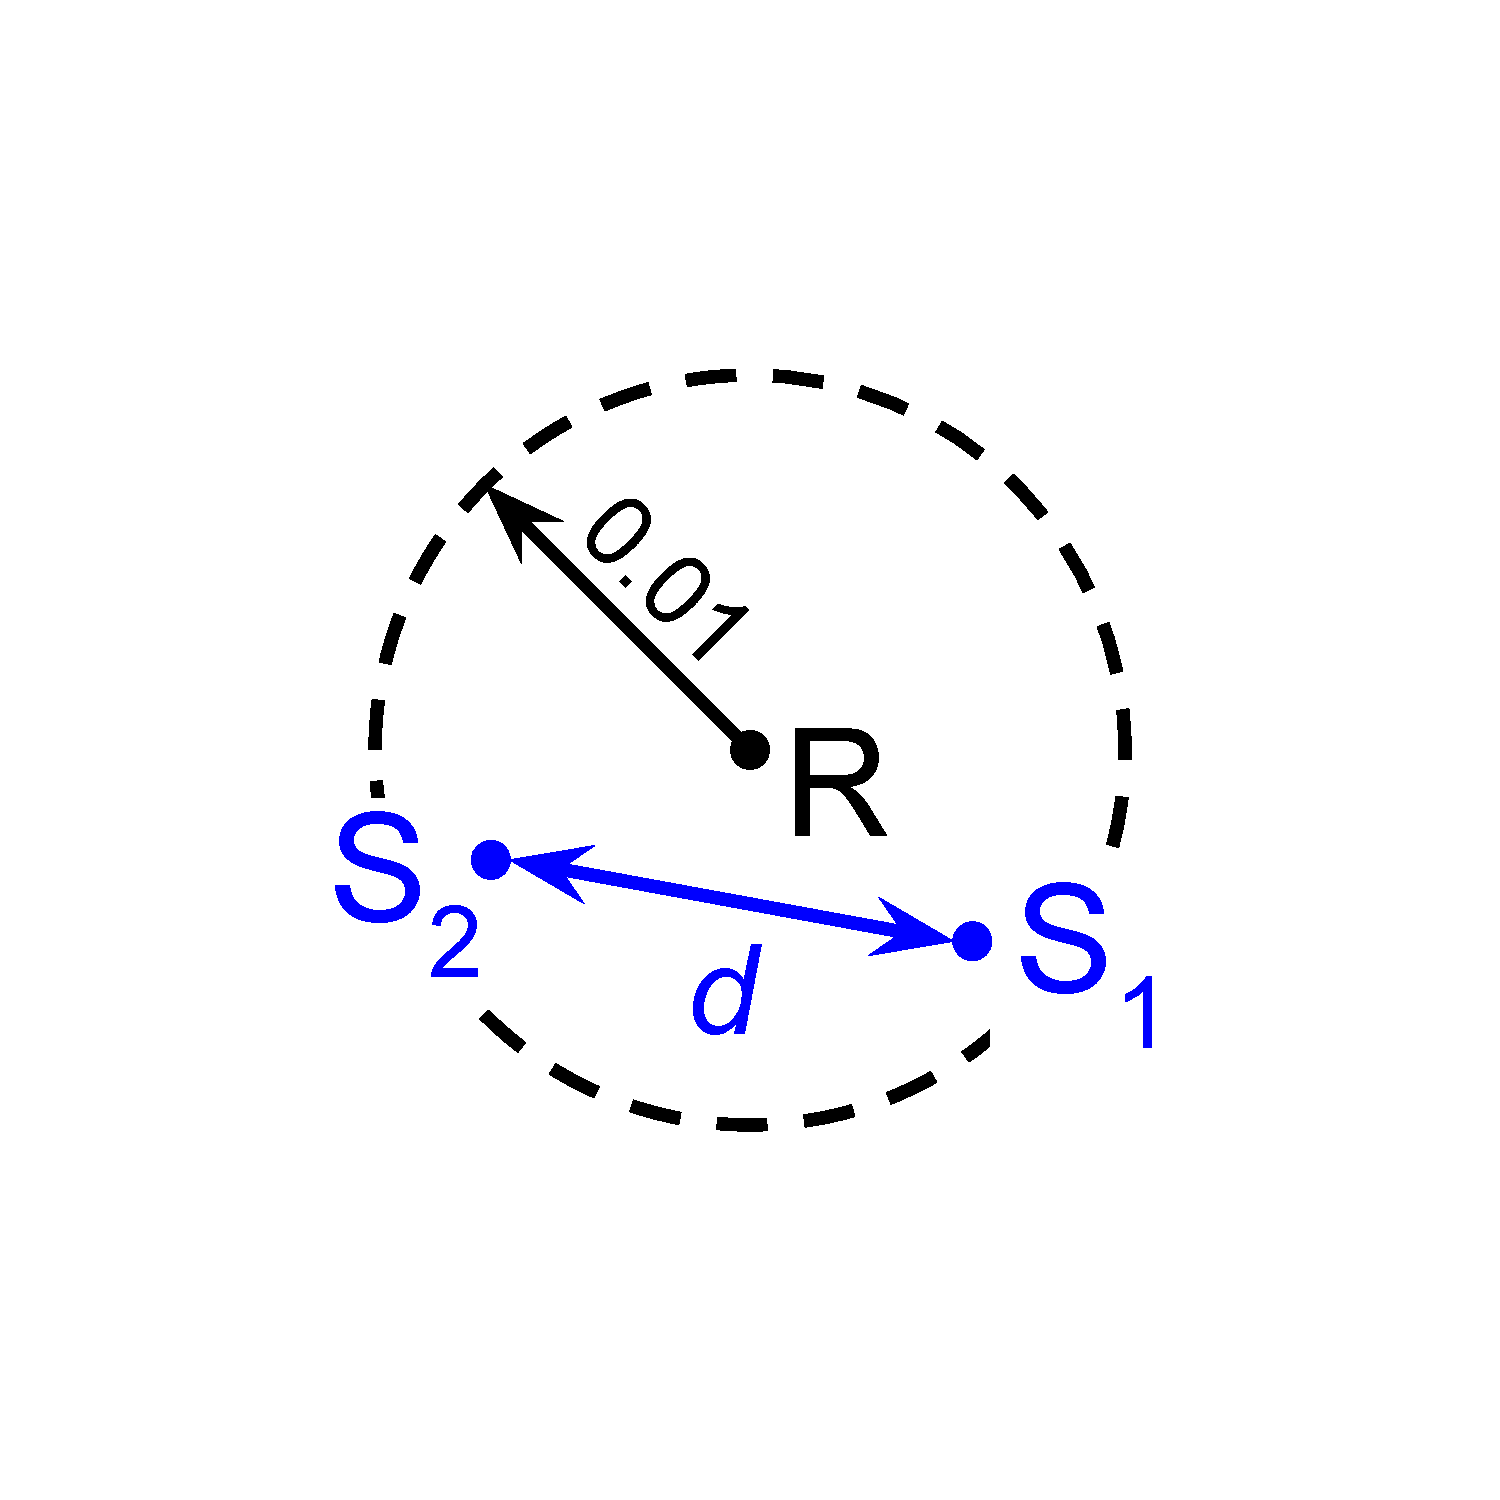
\includegraphics[width=0.5\linewidth,trim=5cm 5cm 5cm 5cm, clip]{img/dimensionality-statistic}
\end{center}
\end{minipage}%
\begin{minipage}{0.5\textwidth}
\caption{
Sampling process used to measure similarity constraint.
First, a constraining tag $R$ was randomly sampled.
Then, tags were randomly drawn until two tags $S_1$ and $S_2$ with distance to $R$ less than 0.01 were obtained.
Finally, similarity constraint was measured as the distance $d$ between $S_1$ and $S_2$.
}
\label{fig:dimensionality_measure}
\end{minipage}
\end{subfigure}
\end{minipage}
\begin{subfigure}[b]{\linewidth}
\begin{minipage}{0.6\linewidth}
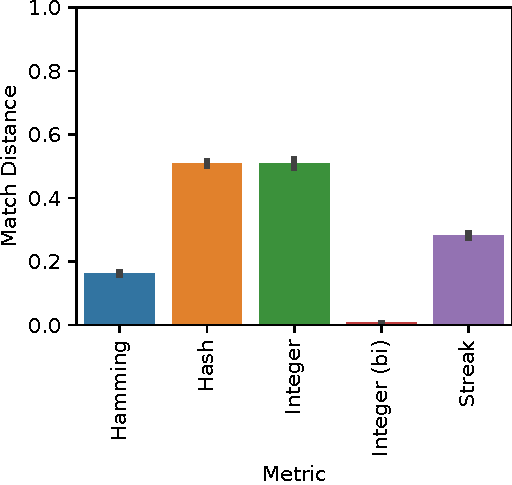
\includegraphics[width=\linewidth]{img/sphere/bitweight=0dot5+seed=1+title=dimensionality_barplot+_data_hathash_hash=c0f6c5cf854ff253+_script_fullcat_hash=03ce1e318a24a109+ext=}
\end{minipage}
\begin{minipage}{0.35\linewidth}
\caption{
Mean similarity constraint.
Error bars represent 95\% confidence intervals.
}
\label{fig:sphere_barplot}
\end{minipage}
\end{subfigure}
\begin{minipage}{\linewidth}
\begin{subfigure}[b]{\linewidth}
\centering
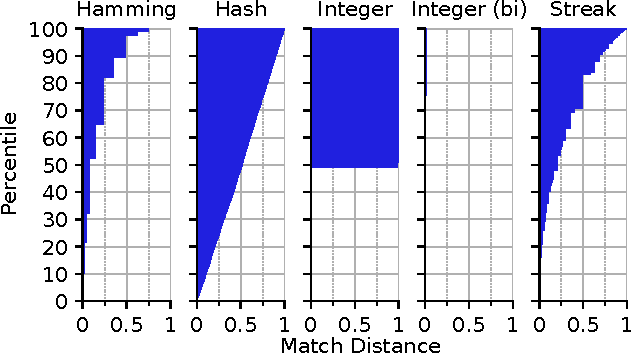
\includegraphics[width=\linewidth]{img/sphere/bitweight=0dot5+seed=1+title=dimensionality_distnplot+_data_hathash_hash=c0f6c5cf854ff253+_script_fullcat_hash=bea2a31376bf6bd0+ext=}
\begin{minipage}{0.8\textwidth}
\caption{
Distributions of sampled similarity constraint values.
Each visualization arranges individually sampled observations (thin horizontal bars) vertically in descending order.
The $y$ axis can be interpreted as ranging form the \nth{0} percentile of outcomes (bottom) to \nth{100} percentile (top) with horizontal bar width showing similarity constraint at a certain percentile.
}
\label{fig:sphere_distnplot}
\end{minipage}
\end{subfigure}
\end{minipage}

\caption{
Similarity constraint of tag-matching metrics.
Figure \ref{fig:dimensionality_measure} summarizes the sampling process used to measure similarity constraint.
Figures \ref{fig:sphere_barplot} and \ref{fig:sphere_distnplot} compare distributions of similarity constraint across metrics.
}
\label{fig:sphere}

\end{center}
\end{figure*}


To characterize similarity constraint, we randomly sampled 5,000 target tags.
Then, for each target tag $R$ we randomly sampled tags until we found two secondarily-sampled tags $S_1$ and $S_2$ that were within a 0.01 match distance radius to the target.
Finally, we computed the match distance $d$ between the pair of secondarily-sampled tags.
Figure \ref{fig:dimensionality_measure} summarizes this process.

Figure \ref{fig:sphere_barplot} provides our estimate of the similarity constraint statistic for each metric, with error bars representing a 95\% confidence interval.
Figure \ref{fig:sphere_distnplot} shows the distribution of the similarity constraint statistic values among the 5,000 replicate samples in greater detail.

In a Euclidean space, similarity constraint corresponds to the average distance between points uniformly sampled from inside a ball (\textit{e.g.}, in two dimensions a circle, in three dimensions a sphere, \textit{etc.}).
In Euclidean space, this average distance increases with dimensionality.
For reference, in a one-dimensional Euclidean space similarity constraint would measure approximately 0.0067.
In a two dimensional Euclidean space, it would measure approximately  0.0091.
In 32 dimensions, it would measure 0.0137 \citep{dunbar1997average}.
So, in some sense, this similarity constraint metric can be interpreted as an indirect measure of dimensionality.
However, as we'll see in Section \ref{sec:detour_difference}, the hamming, hash, and streak metric each impose a decidedly non-Euclidean geometry.

\subsubsection{Bidirectional Integer Metric}

For the bidirectional integer metric, we measured the similarity constraint statistic as 0.0068.
This falls in line with expectation: this metric is essentially identical to a one-dimensional Euclidean space.
As shown in Figure \ref{fig:sphere_distnplot}, the secondarily-sampled match distances are entirely bounded by the diameter of 0.02.
This metric not only exhibits tight similarity constraint in the mean case, but also permits no outliers to the similarity constraint.

\subsubsection{Integer Metric}

The integer metric exhibits much looser similarity constraint in the mean case.
We estimated this value as 0.5092.
However, this looser similarity constraint appears to be an artifact of averaging between two very tight constraints: a tight constraint to 0 in one case and a tight constraint to 1 in the other.
Figure \ref{fig:sphere_distnplot} confirms that all sampled match distances fall under one of these cases.
Because of the asymmetrical definition of the integer metric, half of pairs of similar scalar values will be in ascending order (resulting in a match distance close to 0) and half will be in descending order (resulting in wraparound search and a match distance close to 1).
The integer metric appears to allow for tags closely related to a third tag either very strongly match or very weakly match, but permits no intermediate outcomes.

\subsubsection{Hamming Metric}

The hamming metric exhibits a broader range of sampled similarity constraint values than the integer metrics.
We estimated mean similarity constraint as 0.1627, looser than the bidirectional integer metric.
As shown in Figure \ref{fig:sphere_distnplot}, many secondarily-sampled tag pairs are biased towards low match distances.
However, secondarily-sampled tag pairs that break this constraint are also not uncommon.
Among our 5000 trials, we observed distances between secondarily-sampled tags as high as 0.7499.

Why is our estimate of the hamming metric similarity constraint so much higher than the expected value of 0.0137 in a 32-dimensional Euclidean space?
This phenomenon appears to be due to the normalization process we applied to map raw match distances to a uniform distribution.
We also calculated this statistic for the raw hamming metric without normalization, increasing the radius of our sampling ball to 0.25.
(Only the exact target 32-bit tag itself falls within a sampling radius of 0.01.)
The \textit{a priori} expected distance between sampled points within a 32-dimensional ball with radius 0.25 is 0.3415.
Our estimate of similarity constraint for the raw hamming metric falls nearly in line with expectation at 0.3312.

\subsubsection{Streak Metric}

The streak metric exhibited the next-loosest similarity constraint statistic with a mean value sampled at 0.2813.
For this metric, we observed distances between secondarily-sampled tags as high as 0.9993.
The streak metric retains some geometric constraint in the mean case, but allows for outliers that strongly break similarity constraint.

\subsubsection{Hash Metric}

Like the unidirectional integer metric, the hash metric also exhibits a very loose similarity constraint of 0.5083 in the mean case.
However, unlike the integer metric, secondarily-sampled match distances are uniformly distributed between 0 and 1.
This is exactly as we would expect:
given any particular set of operands, a well-behaved hash function should yield a uniform distribution of hash results.
As expected, the hash metric exhibits no geometric structure.

\subsection{Dissimilarity Constraint} \label{sec:dissimilarityconstraint}

\begin{figure}
\begin{center}

\begin{subfigure}[b]{\columnwidth}
\centering
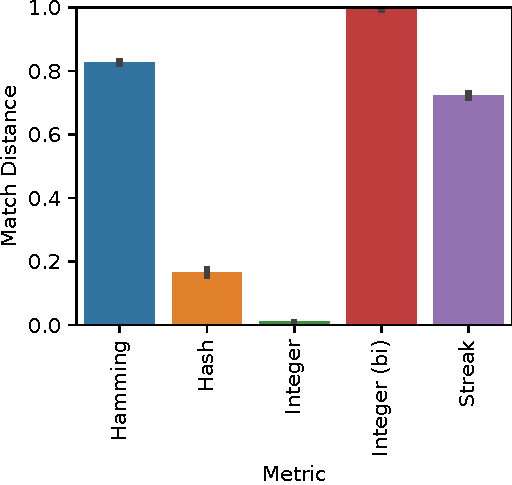
\includegraphics[width=\columnwidth]{{{sphere_reverse/bitweight=0.5+seed=1+title=dimensionality_barplot+_data_hathash_hash=7eaa832497d2f3cb+_script_fullcat_hash=03ce1e318a24a109+ext=}}}
\caption{
TODO
}
\label{fig:sphere_reverse_distnplot}
\end{subfigure}


\begin{subfigure}[b]{\columnwidth}
\centering
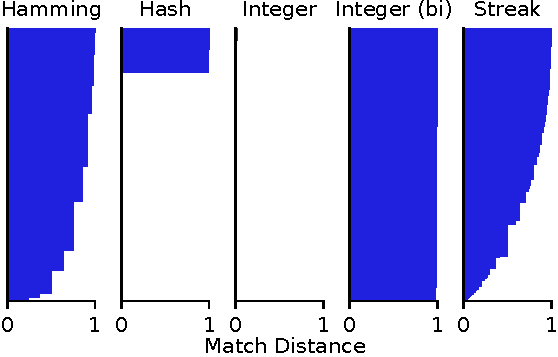
\includegraphics[width=\columnwidth]{{{sphere_reverse/bitweight=0.5+seed=1+title=dimensionality_distnplot+_data_hathash_hash=7eaa832497d2f3cb+_script_fullcat_hash=03ce1e318a24a109+ext=}}}
\caption{
TODO
}
\label{fig:sphere_reverse_barplot}
\end{subfigure}

\caption{
TODO
}
\label{fig:sphere_reverse}

\end{center}
\end{figure}

% \begin{figure}
\begin{center}

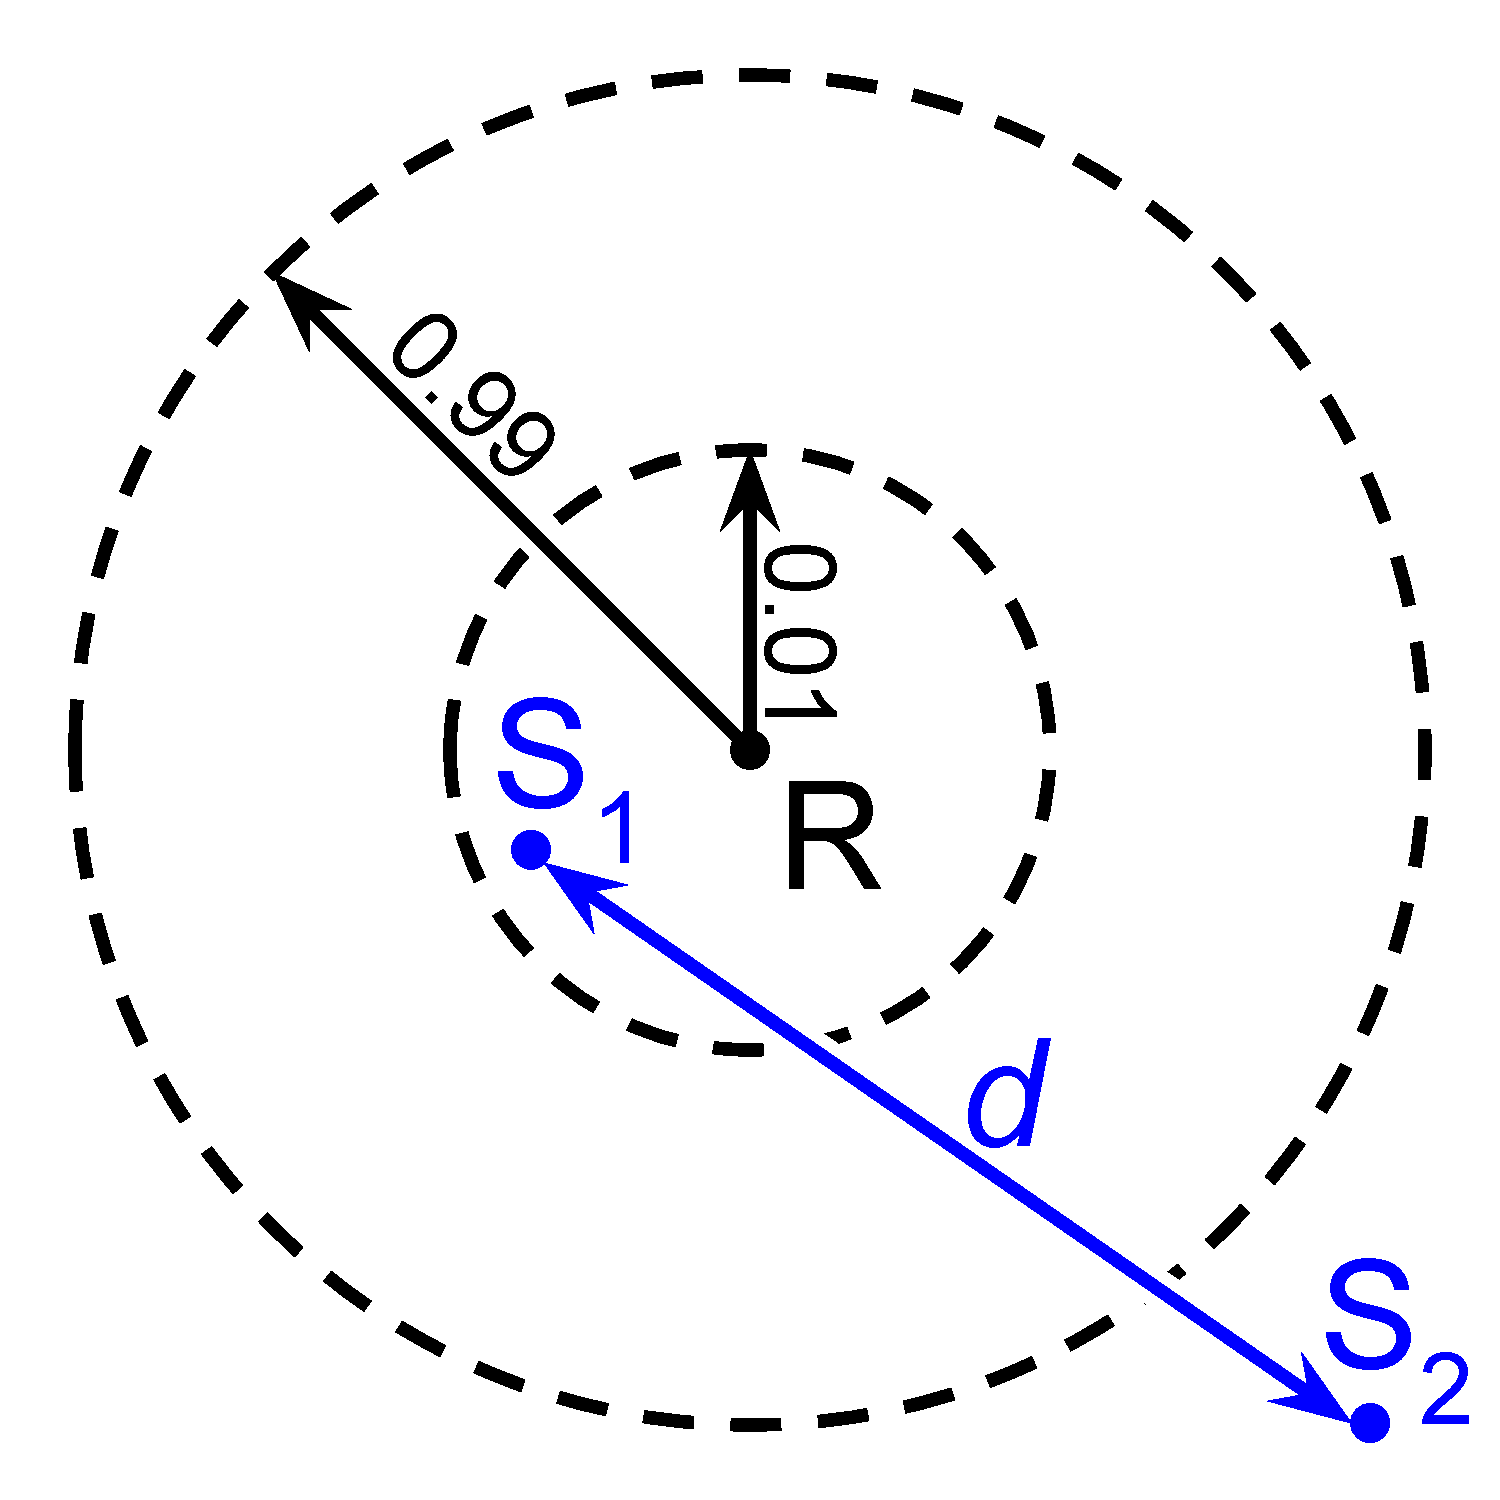
\includegraphics[width=0.5\linewidth]{elasticity-statistic}
\caption{
Dissimilarity statistic
}

\caption{
A schematic depicting the process used to generate the dissimilarity statistic for each metric.
}
\label{fig:dissimilarity_statistic}

\end{center}
\end{figure}


To characterize dissimilarity constraint, we randomly sampled 5,000 target tags.
Then, for each target tag $R$ we randomly sampled tags until we found a secondarily-sampled tag $S_1$ that was within a 0.01 match distance radius of $R$ and a secondarily-sampled tag $S_2$ that was outside a 0.99 match distance radius of the $R$.
Finally, we computed the match distance between $S_1$ and $S_2$.
Figure \ref{fig:dissimilarity_statistic} summarizes this process.

Figure \ref{fig:sphere_barplot} provides our estimate of the dissimilarity constraint statistic for each metric, with error bars representing a 95\% confidence interval.
Figure \ref{fig:sphere_distnplot} shows the distribution of the dissimilarity constraint statistic values among the 5,000 replicate samples in greater detail.

These results tell a similarity to similarity constraint.

\subsubsection{Hash Metric}
The hash metric exhibited no geometric structure --- $S_1$ and $S_2$ were uniformly likely to exhibit any match distance between 0 and 1.

\subsubsection{Streak Metric}

The streak metric exhibited some geometric structure in the mean case. We observed a mean secondarily-sampled distance 0.7127, significantly greater than the mean distance of 0.5 expected between arbitrarily-sampled tags.

However, outcomes that strongly broke geometric constraints also occurred.
We observed distances between secondarily-sampled tags as low as 0.0002.

\subsubsection{Hamming Metric}

The hamming metric exhibited stronger geometric structure in the mean case than the streak metric.
Mean secondarily-sampled distance was 0.8248.

This hamming metric also exhibited less extreme tail-end outcomes than the streak metric.
We observed match distances between the secondarily-sampled tags only as low as 0.2355.

\subsubsection{Bidirectional Integer Metric}

The bidirectional integer metric was highly constrained in both the mean and tail-end cases.
The smallest distance between secondarily-sampled tags observed was 0.9802.

\subsubsection{Integer Metric}

Again, the unidirectional integer metric exhibited a quirky result due to its noncommutative nature.
The mean distance between secondarily-sampled tags was 0.0100.
That is, instead of a bias against close matches as we would expect, secondarily-sampled tags were much closer together than expected under arbitrary sampling.
As shown in Figure \ref{fig:sphere_distnplot}, \textit{all} secondarily-sampled distances observed with this metric were extremely small.
So, although in the opposite way from what we would expect, match distances were still tightly constrained.

The mechanism behind this result stems from the metric's asymmetrical nature.
Under this metric, if you sample a tag that is close to a target it will be numerically slightly larger than the target.
Likewise, if you sample a tag that is very far from a target, it will be numerically slightly smaller than the target (due to wraparound).
Then, explaining this counterintuitive result, the distance from the slightly smaller to the slightly larger tag will be small.

\subsection{Detour Difference} \label{sec:detour_difference}

\begin{figure}
\begin{center}

\begin{minipage}{\linewidth}
\begin{subfigure}[b]{\linewidth}
\begin{minipage}{0.5\textwidth}
\begin{center}
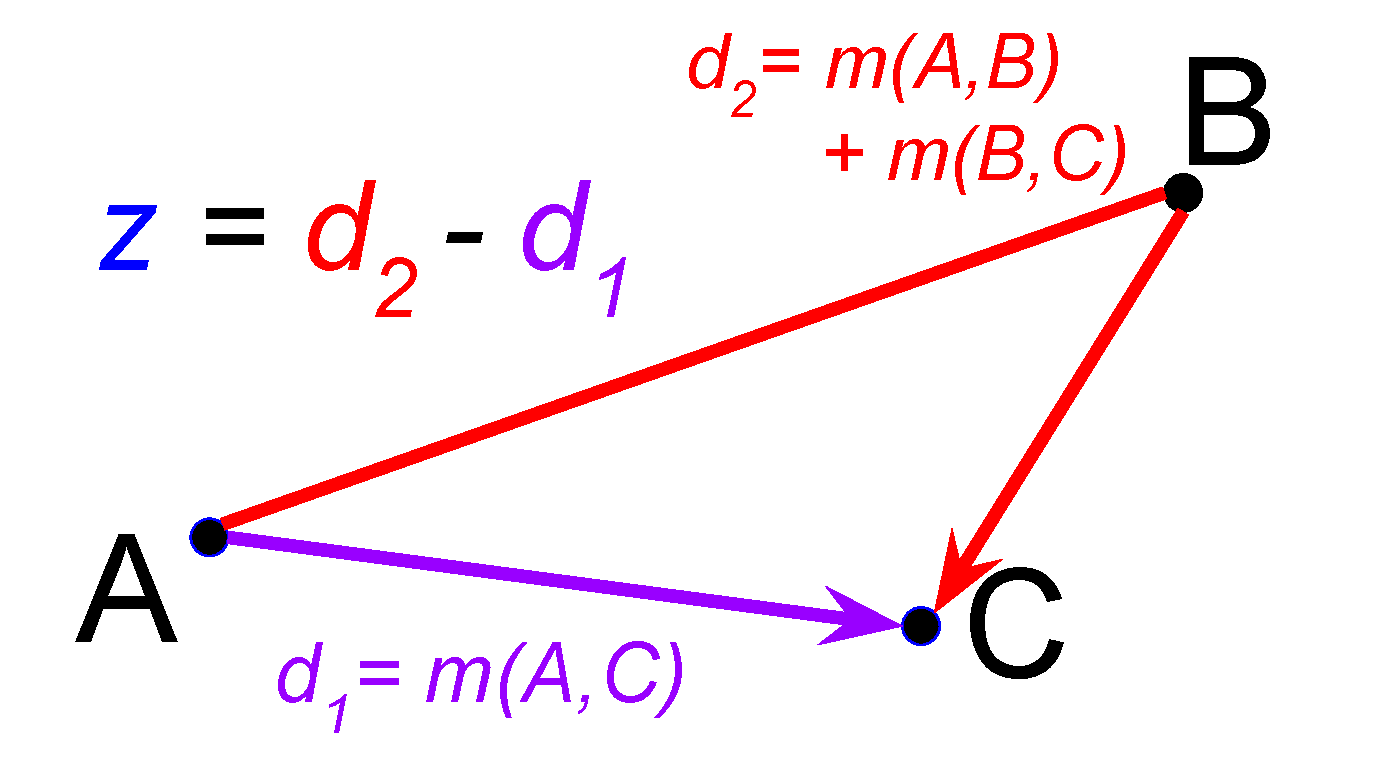
\includegraphics[width=\linewidth,trim=2cm 5cm 2cm 5cm, clip]{detour-difference}
\end{center}
\end{minipage}%
\begin{minipage}{0.5\textwidth}
\caption{
Sampling process used to evaluate detour difference, $z$.
} \label{fig:detour_difference_cartoon}
\end{minipage}
\end{subfigure}
\end{minipage}

\begin{minipage}{\linewidth}
\begin{subfigure}[b]{\linewidth}
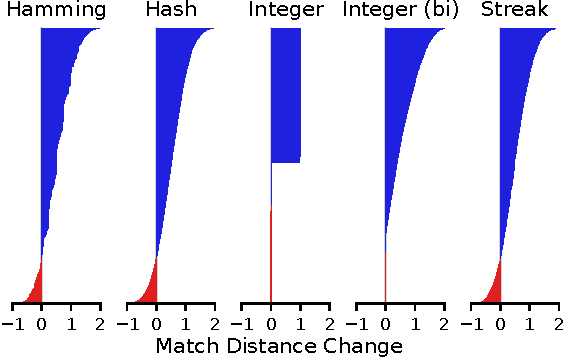
\includegraphics[width=\linewidth]{detour_difference/bitweight=0dot5+seed=1+title=low-triplet-analysis+_data_hathash_hash=6b0749ef97a58721+_script_fullcat_hash=297c4fe09078e17b+ext=}
\caption{
Distributions of detour distance difference for triplets of randomly sampled tags.
Each bar sliver represents an independently sampled observation.
A positive value (colored blue) indicates that total distance increased with the addition of an intermediate stop.
A value of exactly 0 indicates an intermediate stop had no effect on total distance.
A negative value (colored red) indicates violation of the triangle inequality: taking an intermediate stop reduced the total distance travelled.
} \label{fig:detour_difference_distribution}

\end{subfigure}
\end{minipage}

\caption{
Detour difference of tag-matching metrics.
}
\label{fig:detour_difference}

\end{center}
\end{figure}


Similarity constraint and dissimilarity constraint quantify the geometric constraint imposed under preexisting strong matching and strong mismatching, respectively.
To complement these measures, we set out to characterize the regularity, in a loose sense, of each space more broadly.
This led us to our ``detour difference'' measure, which quantifies how tag matching spaces respect the triangle inequality.

Intuitively, detour difference is a measure of how adding a randomly-chosen waypoint affects total distance between a pre-existing start and end.
Under the triangle inequality, the direct route is always shortest.
So, if the triangle inequality is respected, detour difference should always be non-negative.

To measure detour difference, we uniformly sampled 5,000 triplets of tags $A$, $B$, and $C$.
Then, for each metric $m$ we calculated the $m(A, B) + m(B, C) - m(A, C)$.
Figure \ref{fig:detour_difference_cartoon} provides a schematic of this process.

Figure \ref{fig:detour_difference_distribution} plots the distribution of the detour difference statistic for each metric.
The hamming, hash, and streak metrics show evidence of ``shortcuts'' that violate the triangle inequality.\footnote{
The raw hamming metric does respect the triangle inequality, so presumably this result is due to the normalization.
}
Surprisingly, given results from the similarity and dissimilarity constraint measures, the distributions of detour difference for these three metrics appear very similar.
This suggests that geometric differences between these metrics are especially accentuated in contexts of preexisting strong matching and mismatching constraint.


\section{Variational Analysis} \label{sec:variational}

We performed two analyses to characterize the properties of our five match distance metrics under bitwise mutation.
Single-step mutational analysis examines the local mutational neighborhood of tag pairs.
Then, mutational walk analysis surveys the topography of the wider mutational landscape.

\subsection{Single-Step Mutations}

\begin{figure}
\begin{center}

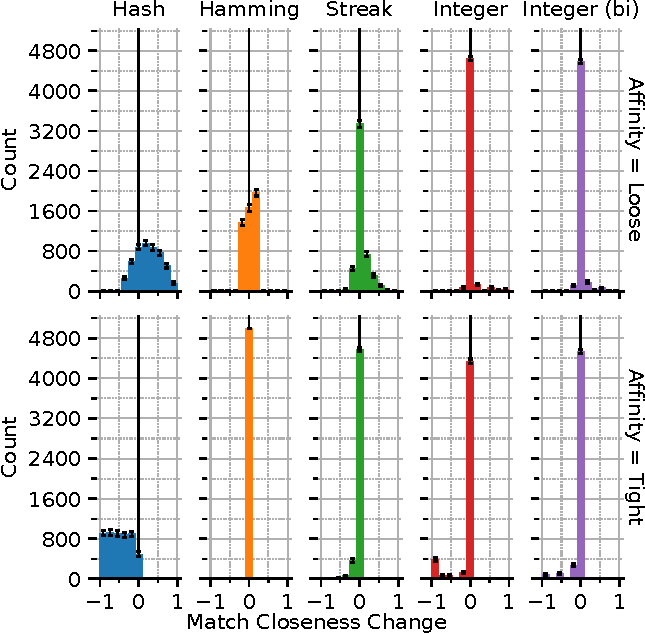
\includegraphics[width=\columnwidth]{img/mutational_step/bitweight=0dot5+seed=1+title=low-mutational-step+viz=hist+_data_hathash_hash=95a57768de56995a+_script_fullcat_hash=aa068ad24b386169+ext=}
\caption{
Distributions of mutation effects on match distance for loosely matched (pre-mutation match distance $> 0.5$) and tightly matched (pre-mutation match distance $< 0.01$) tag pairs.
Note that match closeness change (rather than mast distance change) is plotted so that better-matching mutational outcomes fall to the right and worse-matching mutational outcomes fall to the left.
Error bars are 95\% confidence intervals calculated using the Wilson score method with continuity correction \citep{newcombe1998two}.
Supplementary Figure \ref{fig:mutational_step_supp} shows the cumulative distribution of all sampled match distance changes for each metric.
}
\label{fig:mutational_step}

\end{center}
\end{figure}


Figure \ref{fig:mutational_step} visualizes the distribution of match distance outcomes of single-bit mutations.
We provide this analysis for two categories of tag pairs: tags that were loosely affiliated and tags that were tightly affiliated.

To measure the distribution of mutational perturbations on loosely-affiliated tag pairs we began by sampling a target tag and then randomly sampled candidate tags until we found a second tag with a match distance $> 0.5$.
We recorded the match distance between our tag pair, applied a one-bit mutation to the secondary tag, and then measured the match distance between the tag pair again.
Mutational perturbation was calculated as the difference between the match distances.
A negative mutational perturbation indicates a decrease in match distance and, therefore, an increase in match quality.

We measured the distribution of mutational perturbations on tightly-matched tag pairs similarly, except we uniformly sampled secondary candidate tags until we found a second tag with match distance $< 0.01$.
We sampled 5000 tightly-matched measurements and 5000 loosely-matched measurements for each metric.

For both tightly- and loosely-affiliated tag pairs under the integer and bidirectional integer metrics, most mutations caused very small changes in match distance.
These mutations likely the toggle least-significant bits of the tag's integer representation.
However, under these metrics, a small fraction of mutations affecting more-significant bits of the integer representation have a much stronger effect.
Single-step mutations occassionally occur that strongly couple loosely-affiliated tag pairs or strongly decouple tightly-affiliated tag pairs.
In particular, the unidirectional integer metric, presumably due to its non-commutative quirks, appears to exhibit more frequent strong decoupling mutations than the bidirectional integer metric.

The streak metric is the only metric that exhibits perfectly neutral outcomes under mutation.
These perfectly-neutral mutations presumably affect regions of the bitstring involved neither in the longest-matching streak nor in the longest-mismatching streak.
The streak metric appears to exhibit a fatter tail of match-distance magnitude for mutations that couple loosely-affiliated tags than the integer metrics.
In addition, the most extreme mutational outcomes that couple loosely-affiliated tags appear to be of a comparable magnitude to those under the integer metrics.
Mechanistically, this might be due to mutations that disrupt longest-mismatching streaks.
However, one-step mutations that decouple tightly-affiliated tags do not appear as potent.
This might be because achieving a very poor match requires both increasing longest-mismatching streak length and decreasing longest-matching streak length.

The hamming metric exhibits a generally uniform magnitude of match-distance changes under mutation.
High-magnitude one-step mutations do not occur under this metric.
(Without normalizing match distance to a uniform distribution for randomly-sampled tags, all hamming metric mutations would be of exactly the same magnitude, either increasing or decreasing the count of matching bits by 1).

The hash metric exhibits the fattest tails of mutational magnitude of all metrics.
Extreme-effect one-step mutations are plentiful under this metric.
Interestingly, compared to other metrics, the hash metric exhibits a greater fraction of mutations that decouple tightly-affiliated tags and a greater fraction of mutations that couple loosely-affiliated tags.
This might be due to the hash metric's lack of geometric structure.
Because all one-step mutations uniformly sample a new match distance, 99\% of one-step mutations on tightly-affiliated tags will result in a looser coupling.
Similarly, approximately 75\% of one-step mutations on loosely-affiliated tags will result in a tighter coupling.

\subsection{Mutational Walks}

\begin{figure*}
\begin{center}

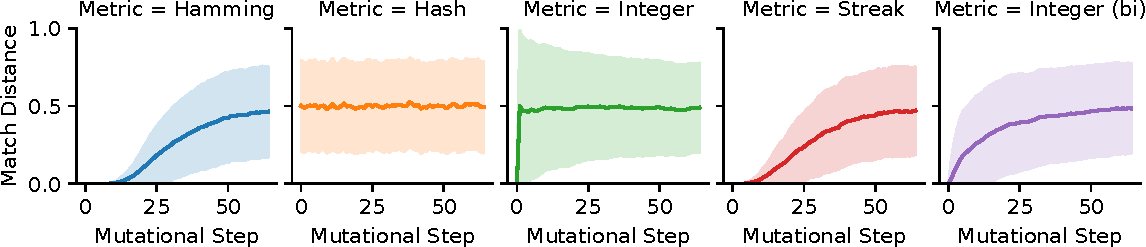
\includegraphics[width=\textwidth]{{{mutational_walk/bitweight=0.5+seed=1+title=mutational_walk_lineplot+_data_hathash_hash=ff15c8831d4f9288+_script_fullcat_hash=c872df869f05035a+ext=}}}
\caption{
TODO
}
\label{fig:mutational_walk_lineplot}

\end{center}
\end{figure*}

\begin{figure}
\begin{center}

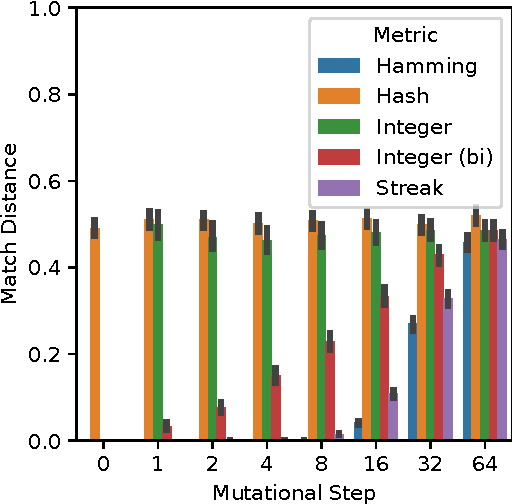
\includegraphics[width=\columnwidth]{{{mutational_walk/bitweight=0.5+seed=1+title=mutational_walk_barplot+_data_hathash_hash=8bf152d87daa9cb7+_script_fullcat_hash=982405ca713eba73+ext=}}}
\caption{
Snapshots of match distance at exponentially increasing steps from identical tags.
Error bars represent 95\% confidence intervals.
}
\label{fig:mutational_walk_barplot}

\end{center}
\end{figure}


Next, we performed mutational walks under each metric.
We began with two randomly chosen equivalent tags (mutation step zero) then applied randomly chosen one-step mutations (with the possibility of back mutation allowed) 65 times to the second tag.
We measured match distance between the two tags at each mutational step.
We performed 1000 independent mutational walks from different starting equivalent tags.

Figure \ref{fig:mutational_walk_lineplot} continuously depicts the distribution of match distances on mutational walks, with shaded areas indicating standard deviation, under different metrics.
Figure \ref{fig:mutational_walk_barplot} compares match distances at exponentially increasing steps.
Error bars indicate 95\% confidence intervals.

For the hash metric, where equivalent tags don't necessarily have low match distance, the mutational walk wanders around loose affinity.

The Spector Integer metric, where half of mutational steps wrap back around to 1.0 distance, immediately spikes up to an average match distance of 0.5.
The variance decreases with mutational steps as the distribution moves away from bias towards distances of 0 and 1.

The bidirectional integer metric experiences a greater immediate jump in variance and significantly greater mean match distance as rare mutations affecting significant bits take place (non-overlapping 95\% CI).

The
Intrestingly, contrary to as was claimed in \citep{downing2015intelligence}, the uniformified streak metric's match score under mutation actually grows significantly faster than the hamming metric's match score  (non-overlapping 95\% CI).

Because the are uniformified, the distributions all devolve to having an equivalent mean and variance.




\section{Evolutionary Analysis}

\begin{figure}
% \begin{minipage}{6in}
\begin{center}

\begin{minipage}{0.05\textwidth}
~
\end{minipage}%
\begin{minipage}{0.95\textwidth}
\begin{minipage}{0.05\textwidth}
~
\end{minipage}%
\begin{minipage}{0.95\textwidth}
\centering
\large
\textbf{Mean Degree}
\end{minipage}
\begin{minipage}{0.05\textwidth}
~
\end{minipage}%
\begin{minipage}{0.95\linewidth}
\begin{minipage}{0.5\textwidth}
\centering
\large
1
\end{minipage}%
\begin{minipage}{0.5\textwidth}
\centering
\large
2
\end{minipage}
\end{minipage}
\end{minipage}\\
\vspace{2ex}





\begin{minipage}{0.05\textwidth}
\large
\rotatebox[origin=c]{90}{\textbf{Structure}}
\end{minipage}%
\begin{minipage}{0.95\textwidth}
\begin{minipage}{0.05\linewidth}
\large
\rotatebox[origin=c]{90}{Irregular}
\end{minipage}%
\begin{minipage}{0.95\linewidth}
\begin{subfigure}[b]{0.5\textwidth}
\centering
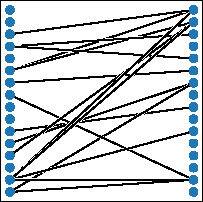
\includegraphics[width=\textwidth]{img/graph_layouts/title=irregular-1+ext=}%
\caption{
Irregular w/ mean degree 1
}
\label{fig:irregular_1}
\end{subfigure}
\begin{subfigure}[b]{0.5\textwidth}
\centering
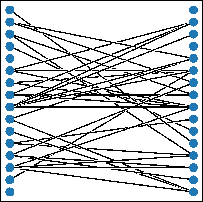
\includegraphics[width=\textwidth]{img/graph_layouts/title=irregular-2+ext=}%
\caption{
Irregular w/ mean degree 2
}
\label{fig:irregular_2}
\label{fig:irregular_degree_2}
\end{subfigure}

\end{minipage}

\vspace{2ex}

\begin{minipage}{\textwidth}

\begin{minipage}{0.05\linewidth}
\large
\rotatebox[origin=c]{90}{Regular}
\end{minipage}%
\begin{minipage}{0.95\linewidth}
\begin{subfigure}[b]{0.5\textwidth}
\centering
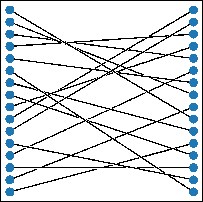
\includegraphics[width=\textwidth]{img/graph_layouts/title=regular-1+ext=}%
\caption{
Regular w/ mean degree 1
}
\label{fig:regular_degree_1}
\label{fig:regular_1}
\end{subfigure}
\begin{subfigure}[b]{0.5\textwidth}
\centering
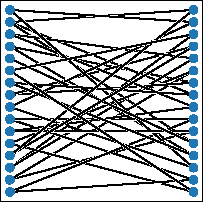
\includegraphics[width=\textwidth]{img/graph_layouts/title=regular-2+ext=}%
\caption{
Regular w/ mean degree 2
}
\label{fig:regular_degree_2}
\label{fig:regular_2}
\end{subfigure}
\end{minipage}
\end{minipage}
\end{minipage}

\caption{
Example target graph layouts used in 32-node graph-matching evolutionary experiments.
Blue dots represent tagged nodes.
Black lines represent selected-for tight affinity relationships.
Layouts differ in total number of selected-for affinities (``mean degree'') and whether selected-for affinities were evenly or randomly distributed between nodes (``structure'').
}
\label{fig:graph_layouts}


\end{center}
% \end{minipage}
\end{figure}


fitness function was based on rank matching.
Randomly generated bipartite graph as a target.
Degree, which refers to the mean number of edges attached to each node.
Regular edges were generated by randomly connecting the bipartite graph such that all left nodes and all right nodes had the same number of connections.
Irregular edges were generated by randomly adding left to right connections.
In this case, some left nodes may have more than the mean degree of edges and some left nodes may have no or fewer than the mean degree of edges.
Likewise for right nodes.
Figure \ref{fig:graph_layouts} depicts these graph layouts.

Genomes consisted of bitstring tags, sixteen representing left nodes in the bipartite graph and sixteen representing right nodes.
To evaluate the fitness of a genome, we harvested the right node tags and placed them in a tag-matching data structure that returns the ranked ordering of tag matches for a particular query tag.
Then, queried the tag-matching data structure with each left node tag in the genome.
We cut down the ranked ordering list returned to the number of the left node tag's outgoing connections in the bipartite target graph.
Fitness was calculated as the fraction of these remaining right node results that corresponded to edges in the bipartite target graph.

We performed 512-generation evolutionary runs with population size 500 and tournament size 7.
We tested combinations of two target graph types: irregular/regular edge layout and mean degree 1 or mean degree 2.
For each configuration, we surveyed each metric's performance over ten per-bit mutation rates ranging from 0.75 expected mutations per genome to 16.0 expected mutation rates per genome.
(Supplementary Figure \ref{fig:evolve_mutsweep} summarizes these results, confirming that each metric/target graph configuration shows a local maximum of performance within the range of mutation rates surveyed.)
For each metric and target graph configuration combination, we chose the most favorable mutation rate defined by sum population-maximum fitness across updates.
We ran 100 replicate evolutionary runs for each mutation rate/target graph/metric combination.

\begin{minipage}{\linewidth}
\begin{center}

\begin{minipage}{\linewidth}
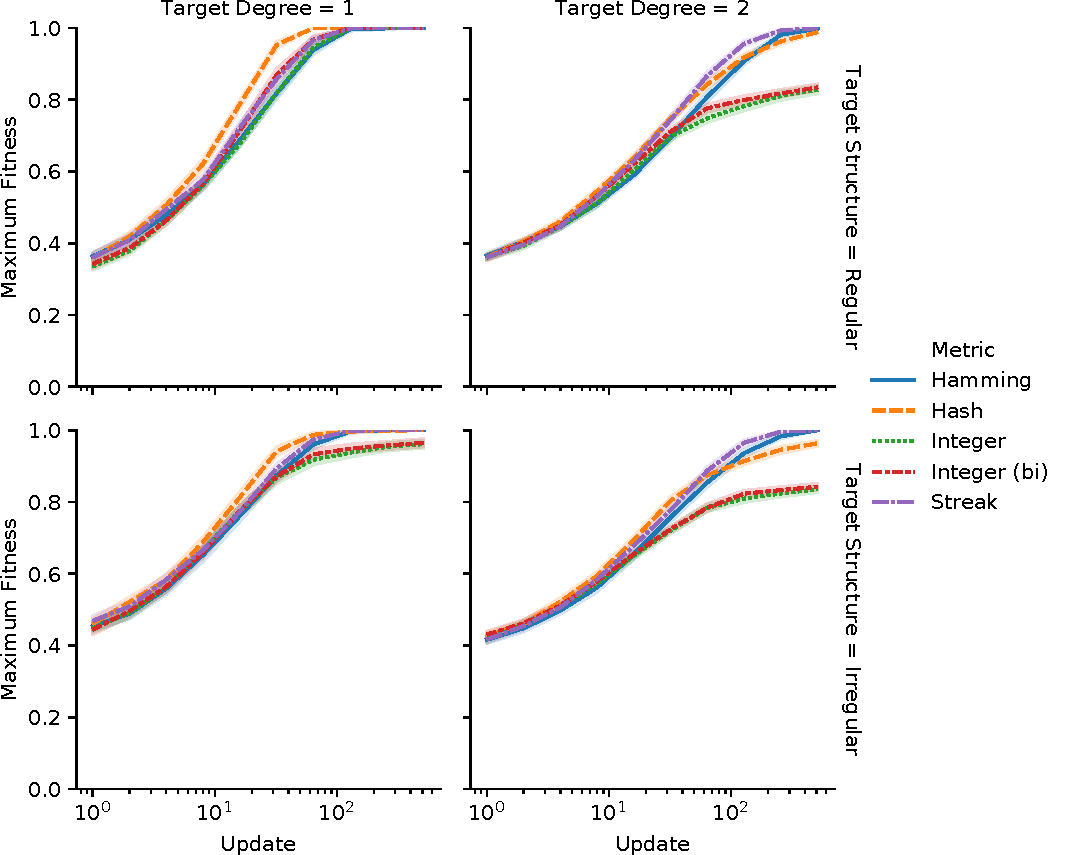
\includegraphics[width=\linewidth]{target_evolve/viz=max-fitness-line+_data_hathash_hash=673d309ab90e91d1+_script_fullcat_hash=fe3ddc711c5abfad+ext=}
\end{minipage}
\begin{minipage}{\linewidth}
\caption{
Maximum fitness by update over replicate runs for each metric's best-performing mutation rate.
Note log-scale x-axes.
Shaded area represents 95\% confidence intervals.
}
\label{fig:evolve_bests}
\end{minipage}
\end{center}
\end{minipage}


Figure \ref{fig:evolve_bests} plots population-maximum fitness across evolutionary runs.
Unsurprisingly, the hash metric performs much more poorly than all other metrics (non-overlapping 95\% confidence intervals).
The integer metrics are capable of evolving solutions to the one-to-one matching problem of the mean degree 1, regular target graph.
However, on mean degree 2 target graphs they evolve significantly poorer quality solutions.

The streak metric performs favorably or equivalently compared to all other metrics across all target graph configurations.
The streak metric yields significantly more rapid adaptive evolution than all other metrics on the regular mean degree 2 graph (non-overlapping 95\% CI).




\section{Discussion}

% \begin{figure}
\begin{center}

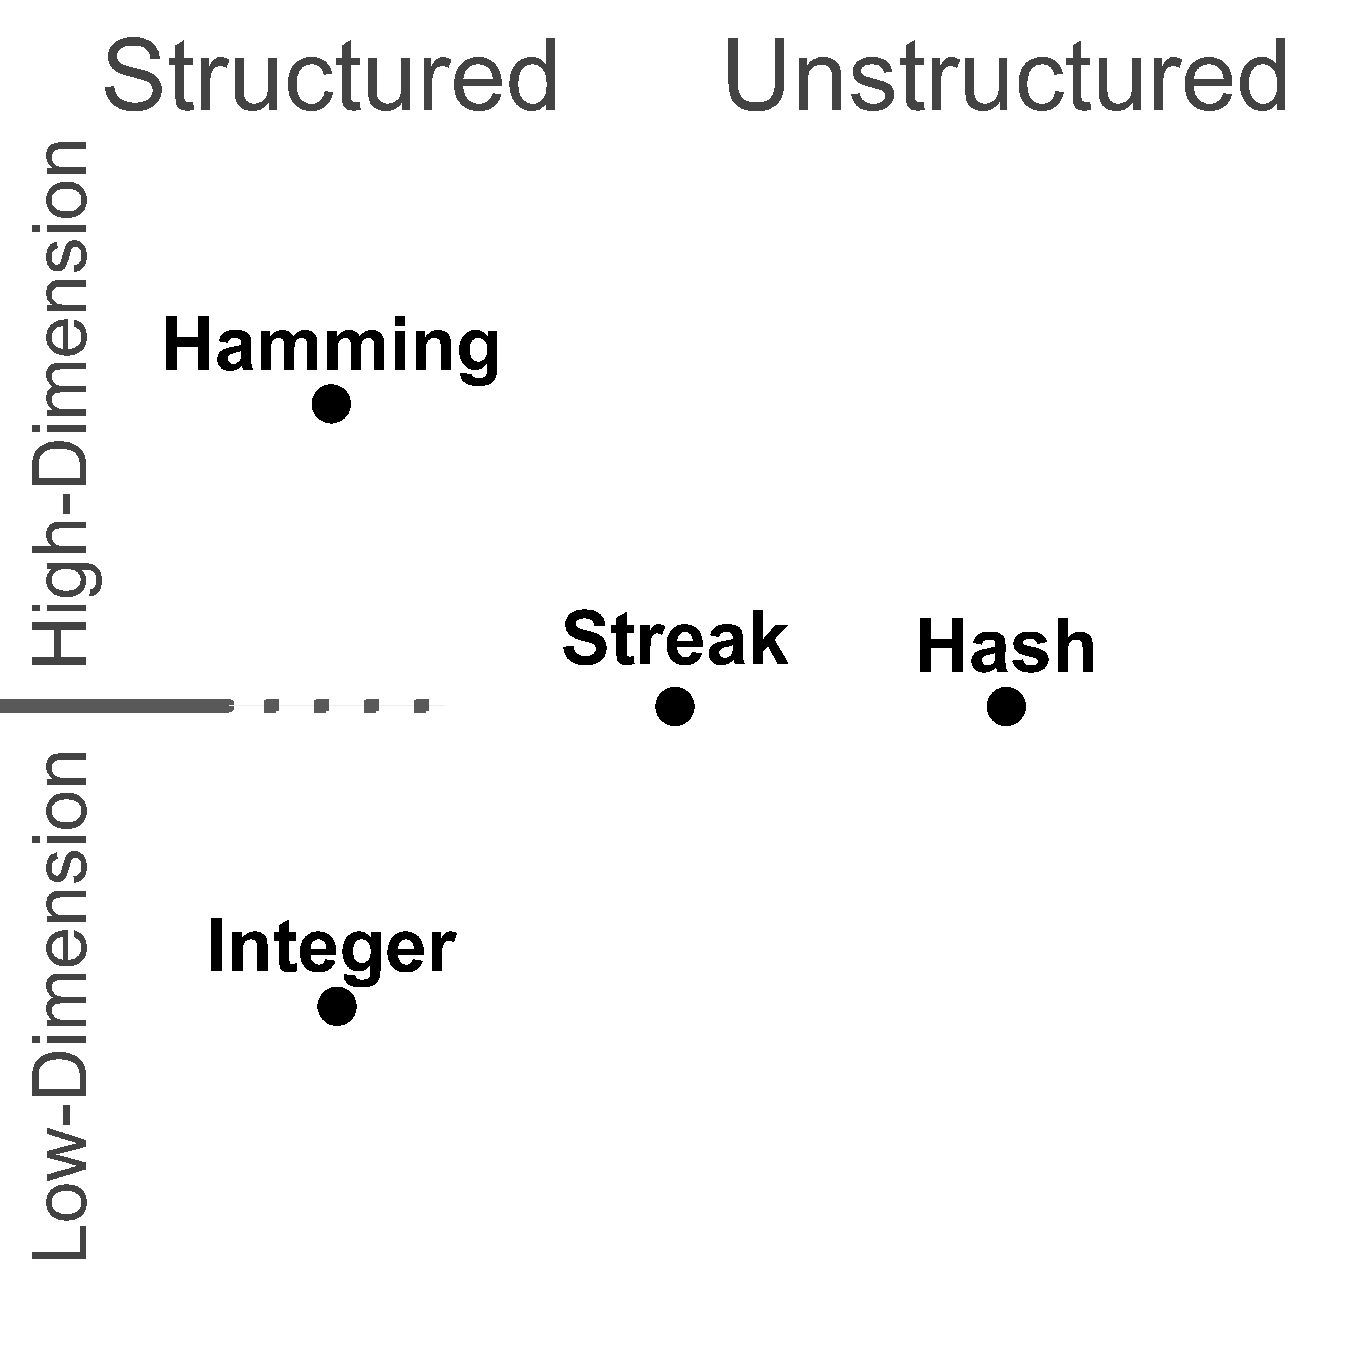
\includegraphics[width=\columnwidth]{{{img/conceptual-geometry}}}
\caption{
A conceptual schematic of the tag-matching metrics' geometric properties.
}
\label{fig:conceptual_geometry}

\end{center}
\end{figure}

First, we performed geometrical analyses to understand how our panel of tag-matching metrics constrain the patterns of that tend to, or even are possible to, arise.
If two tags both closely match a third tag, will these two tags be constrained to closely match each other?
Likewise, if a tag closely matches a second tag, will the tag be constrained to poorly match other tags the second tag poorly matches?

We found that the bidirectional integer metric exhibited the tightest geometrical constraint in our analyses.
The unidirectional integer metric also exhibits tight geometrical constraint, but quirks of its non-commutative construction allows that constraint to split across extremes of poor- and close-matching.
Hamming and streak metrics are more loosely constrained, with the streak metric allowing for edge cases that very strongly break geometric constraint.
Finally, the hash metric exhibits no geometrical structure or constraint.

Next, we analyzed the effect of bitwise mutation on match distance score under the different metrics.
Under the hamming metric, all mutations have small effects on match distance score.
In contrast, under the integer metrics, rare mutations have strong effects on match distance score.
The streak metric also exhibited strong-effect mutations, particularly on coupling loosely-affiliated tags.
The hash metric exhibited the fattest tails of mutational effect, with strong-effect mutations occuring frequently.
Interestingly, the hash metric also exhibited sign-outcome frequencies that differed from the other metrics.
Mutations that decoupled tightly-matching tags and mutations that coupled loosely-matching tags were more frequent.

On mutational walks from an identical tag pair, the hamming metric exhibited the greatest robustness to mutation, followed by the streak metric.
The integer metrics, in particular the unidirectional integer metric, exhibted less robustness.
The streak metric, where all one-step mutations scramble match distance, exhibited the least robustness.

In target-matching evolutionary experiments, we found that the hash metric enabled rapid adaptive evolution towards targets with low tag-matching constraint.
This rapid evolution may be due to the hash metric's ability to rapidly generate variation.
In cases with high tag-matching consraint, however, the hash metric yielded poor-quality solutions.
The integer metrics also yielded poor-quality solutions for targets with tag-matching constraint.
In some more-constrained cases, the streak metric enabled more rapid adaptive evolution than the hamming metric.

In evolutionary experiments to evolve genetic programs, we found that the hamming and streak metrics yielded successful solutions the most frequently.
The hash metric had the next best performance, yielding more solutions than the integer metrics, which performed comparably.
Interestingly, on the directional signal task, which tends to evolve networks with more tag-matching constraints (high-degree regualation/activation interaction network) we found evidence that the streak metric enabled more rapid adaptive evolution than the hamming metric.

The streak metric seems to offer variational and geometric properties that are in many ways intermediate between the hash metric and the integer and hamming metrics.
It exhibits low, but some, geometric constraint.
Many mutations are neutral (like the integer metrics) but extreme-effect mutations also occur.
However, it is unclear exactly why it enabled more rapid adaptive evolution on the genetic programming problem.





\section{Conclusion}

Better understanding the mechanistic properties and functional implications of tag-matching criteria will help artificial life practitioners more effectively incorporate tag matching in model systems and better understand the biases imposed by those criteria.
In particular, our analyses suggests that network constraint (i.e., the degree of connectivity networks constructed by tag matching) is key to the interaction between a tag-matching scheme and problem domain.
% Better understanding tag-matching criteria willOutside of artificial life, particularly in genetic programming, where increasing the rate of adaptive evolution and evolving better-quality solutions is a key concern.

However, open questions remain with respect tag-matching criteria.
In particular, the relationships between tag-matching criteria and specificity, modularity, robustness, and the process of duplication and divergence should be explored. 
Evolvability or information-theoretical analyses may prove fruitful in this regard \citep{tarapore2015evolvability}.
How to 
%apply insight into tag-matching criteria to 
systematically design new tag-matching metrics with desirable properties also remains an open problem.

Tag-like mechanisms play a central role mediating interaction and function across the spectrum of biological scale \citep{holland2012signals}.
% Our work suggests that tag-matching systems  can have implications with respect to the structure and evolution of interaction networks.
By shining light on previously-unexplored mechanistic and evolutionary properties of tagging systems, we hope that insight into artificial tag models will translate into a more nuanced appreciation of natural systems.


% \section{Software and Data Availability}

We implemented our experimental systems using the Empirical library for scientific software development in C++, available at \url{https://github.com/devosoft/Empirical} \citep{charles_ofria_2019_2575607}.
The code used to perform and analyze our experiments, our figures, and data from our experiments is available via the Open Science Framework at \url{https://osf.io/gw5mc/} \citep{foster2017open}.


\section{Acknowledgements}

Thanks to members of the DEVOLAB, in particular TODO for help with TODO.
This research was supported in part by NSF grants DEB-1655715 and DBI-0939454, and by Michigan State University through the computational resources provided by the Institute for Cyber-Enabled Research.
This material is based upon work supported by the National Science Foundation Graduate Research Fellowship under Grant No. DGE-1424871.
Any opinions, findings, and conclusions or recommendations expressed in this material are those of the author(s) and do not necessarily reflect the views of the National Science Foundation.


\footnotesize
\bibliographystyle{apalike}
\bibliography{bibl} % replace by the name of your .bib file

\clearpage
\newpage

\newgeometry{left=0.5in,right=0.5in,top=1in,bottom=1in}

\appendix

\setcounter{secnumdepth}{2}

\section{Supplementary Materials}

\begin{figure}[]{\linewidth}
\centering
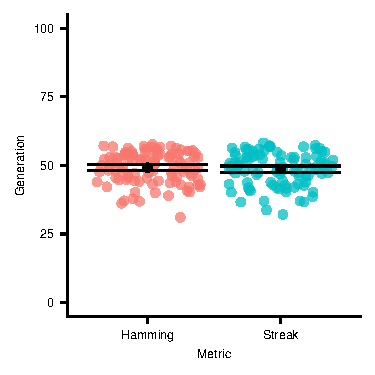
\includegraphics[width=\linewidth]{img/gp_results/panel-cst-times.pdf}%
\caption{
 CST TODO
 }
\label{fig:cst-times}
\end{figure}


\begin{figure*}
\begin{minipage}{6in}
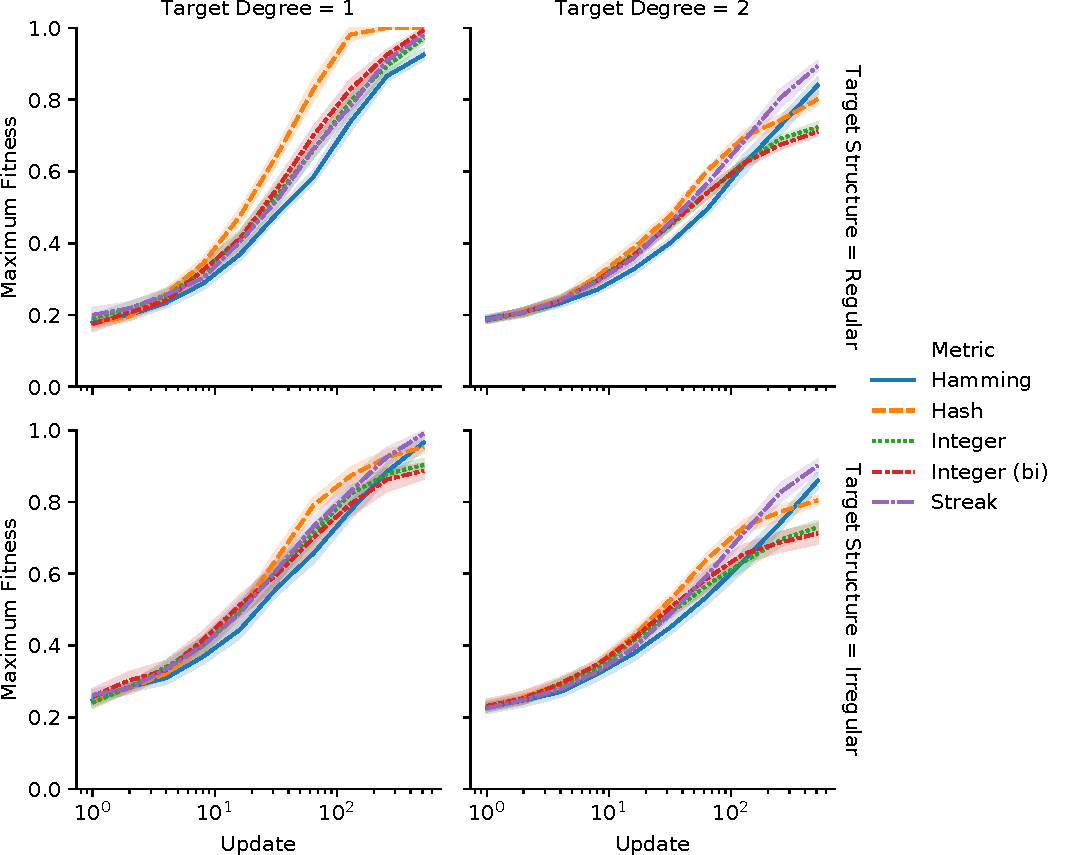
\includegraphics[width=\textwidth]{img/target_evolve_big/viz=max-fitness-line+_data_hathash_hash=4db1200f9d71a980+_script_fullcat_hash=fe3ddc711c5abfad+ext=}
\caption{64-node target graph}
\label{fig:evolve_big_bests}
\end{minipage}
\begin{minipage}{\textwidth}
\caption{
Trajectories of adaptive evolution for each tag-matching metric on the 64-node graph-matching task.
Maximum fitness represents the best fitness value for any individual within a population.
Here report using each metric's best-performing per-bit mutation rate.
(See Supplementary Figure \ref{fig:evolve_big_mutsweep} for survey showing how mutation rate affects adaptive evolution under each metric.)
Note log-scale x-axes.
Shaded area represents bootstrapped 95\% confidence intervals across 20 replicate observations.
}
\label{fig:evolve_bests64}
\end{minipage}
\end{figure*}


\begin{figure}
% \begin{minipage}{6in}
\begin{center}

\begin{minipage}{0.05\textwidth}
~
\end{minipage}%
\begin{minipage}{0.95\textwidth}
\begin{minipage}{0.05\textwidth}
~
\end{minipage}%
\begin{minipage}{0.95\textwidth}
\centering
\large
\textbf{Mean Degree}
\end{minipage}
\begin{minipage}{0.05\textwidth}
~
\end{minipage}%
\begin{minipage}{0.95\linewidth}
\begin{minipage}{0.5\textwidth}
\centering
\large
1
\end{minipage}%
\begin{minipage}{0.5\textwidth}
\centering
\large
2
\end{minipage}
\end{minipage}
\end{minipage}\\
\vspace{2ex}





\begin{minipage}{0.05\textwidth}
\large
\rotatebox[origin=c]{90}{\textbf{Structure}}
\end{minipage}%
\begin{minipage}{0.95\textwidth}
\begin{minipage}{0.05\linewidth}
\large
\rotatebox[origin=c]{90}{Irregular}
\end{minipage}%
\begin{minipage}{0.95\linewidth}
\begin{subfigure}[b]{0.5\textwidth}
\centering
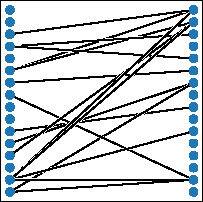
\includegraphics[width=\textwidth]{img/graph_layouts/title=irregular-1+ext=}%
\caption{
Irregular w/ mean degree 1
}
\label{fig:irregular_1}
\end{subfigure}
\begin{subfigure}[b]{0.5\textwidth}
\centering
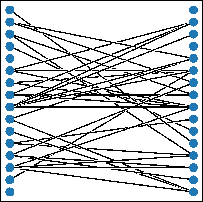
\includegraphics[width=\textwidth]{img/graph_layouts/title=irregular-2+ext=}%
\caption{
Irregular w/ mean degree 2
}
\label{fig:irregular_2}
\label{fig:irregular_degree_2}
\end{subfigure}

\end{minipage}

\vspace{2ex}

\begin{minipage}{\textwidth}

\begin{minipage}{0.05\linewidth}
\large
\rotatebox[origin=c]{90}{Regular}
\end{minipage}%
\begin{minipage}{0.95\linewidth}
\begin{subfigure}[b]{0.5\textwidth}
\centering
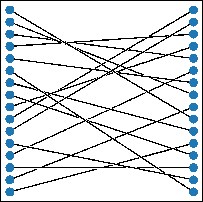
\includegraphics[width=\textwidth]{img/graph_layouts/title=regular-1+ext=}%
\caption{
Regular w/ mean degree 1
}
\label{fig:regular_degree_1}
\label{fig:regular_1}
\end{subfigure}
\begin{subfigure}[b]{0.5\textwidth}
\centering
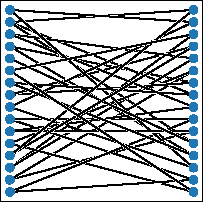
\includegraphics[width=\textwidth]{img/graph_layouts/title=regular-2+ext=}%
\caption{
Regular w/ mean degree 2
}
\label{fig:regular_degree_2}
\label{fig:regular_2}
\end{subfigure}
\end{minipage}
\end{minipage}
\end{minipage}

\caption{
Example target graph layouts used in 32-node graph-matching evolutionary experiments.
Blue dots represent tagged nodes.
Black lines represent selected-for tight affinity relationships.
Layouts differ in total number of selected-for affinities (``mean degree'') and whether selected-for affinities were evenly or randomly distributed between nodes (``structure'').
}
\label{fig:graph_layouts}


\end{center}
% \end{minipage}
\end{figure}


\begin{figure*}
\begin{center}

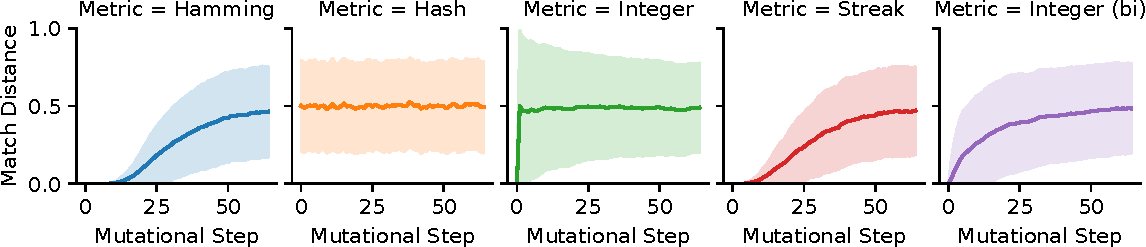
\includegraphics[width=\textwidth]{{{mutational_walk/bitweight=0.5+seed=1+title=mutational_walk_lineplot+_data_hathash_hash=ff15c8831d4f9288+_script_fullcat_hash=c872df869f05035a+ext=}}}
\caption{
TODO
}
\label{fig:mutational_walk_lineplot}

\end{center}
\end{figure*}


\begin{figure}
\begin{center}

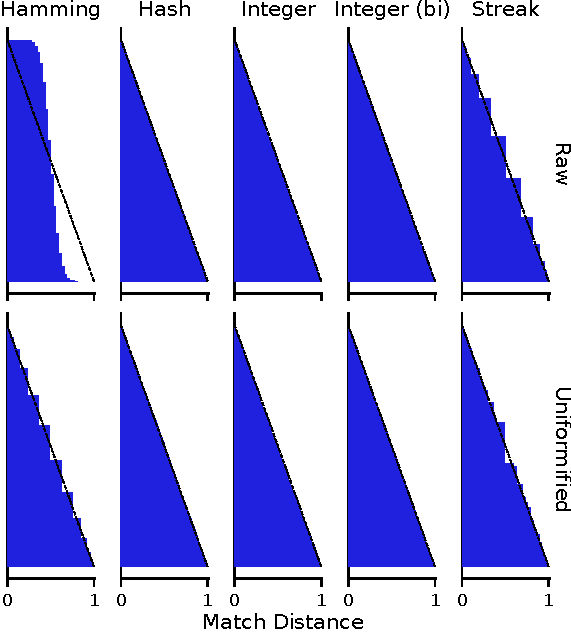
\includegraphics[width=\columnwidth]{img/uniformification/bitweight=0dot5+seed=1+title=low-score-distribution+_data_hathash_hash=75684cf1e73fb7f1+_script_fullcat_hash=d4b3b5e14a0d1350+ext=}
\caption{
Distance distributions of metrics before and after uniformification.
Dashed line indicates an ideal uniform distribution.
}
\label{fig:uniformification}

\end{center}
\end{figure}


\begin{figure*}[!htbp]
\begin{minipage}{6in}
\begin{center}

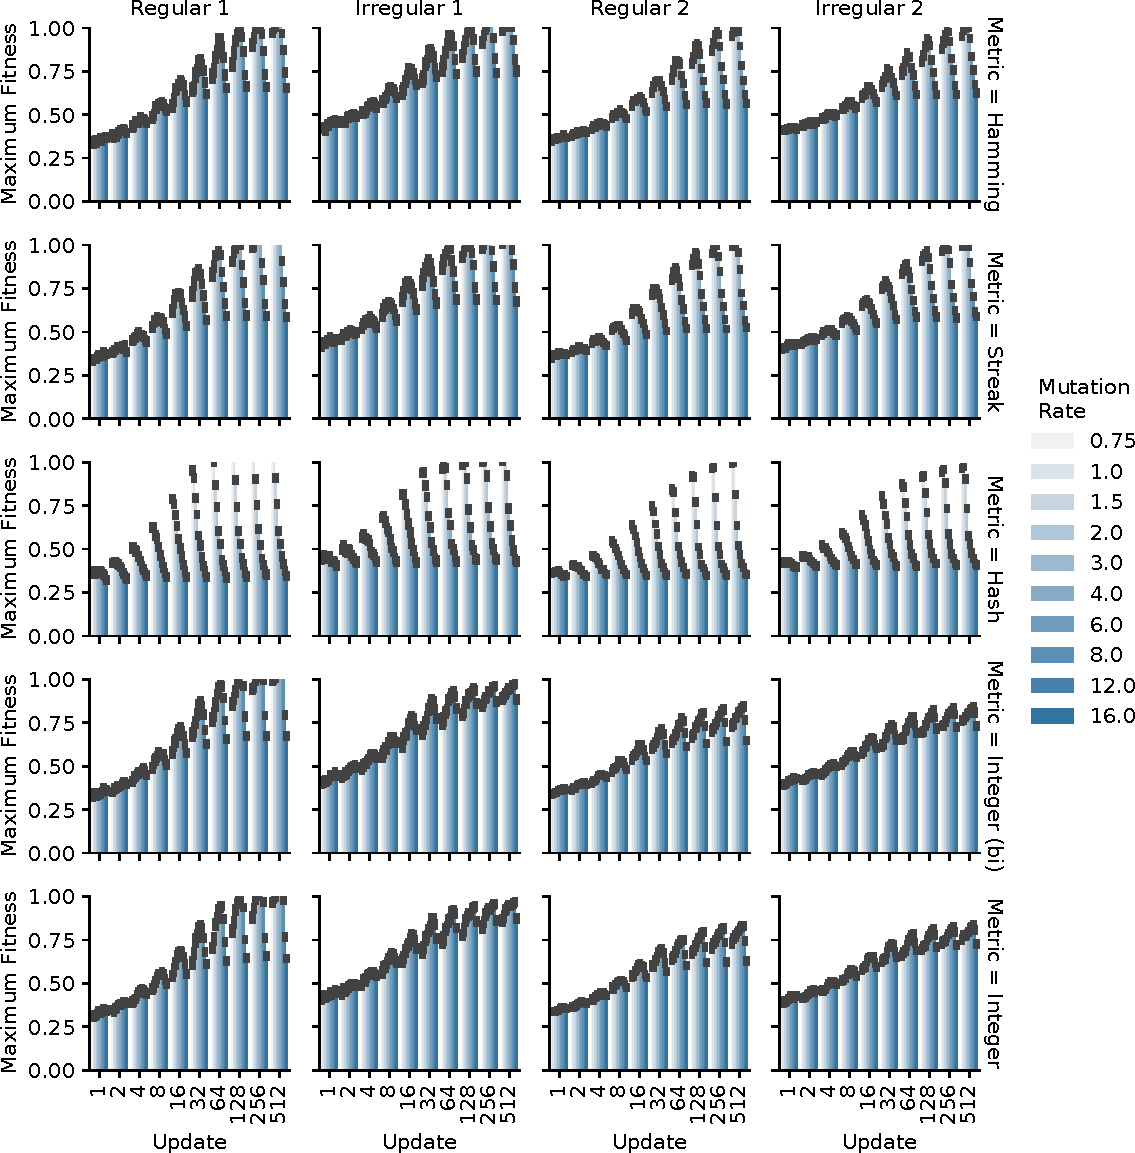
\includegraphics[width=\textwidth]{img/target_evolve/title=fitness_mutation_barplot+_data_hathash_hash=4c78832f20b46ffd+_script_fullcat_hash=6ccad43c80699be8+ext=}
\caption{
32-node graph-matching task mutation rate sensitivity analysis.
Metrics exhibited fastest adaptive evolution within the range of mutation rates surveyed, except the hash metric which exhibited fastest adaptive evolution at at the lowest mutation rate surveyed.
Maximum fitness is the best fitness value for any individual within a population.
Maximum fitness at each update is presented across the range of surveyed mutation rates.
Error bars represent bootstrap 95\% confidence intervals across 50 replicate populations.
}
\label{fig:evolve_mutsweep}

\end{center}
\end{minipage}
\end{figure*}


\begin{figure*}
\begin{center}

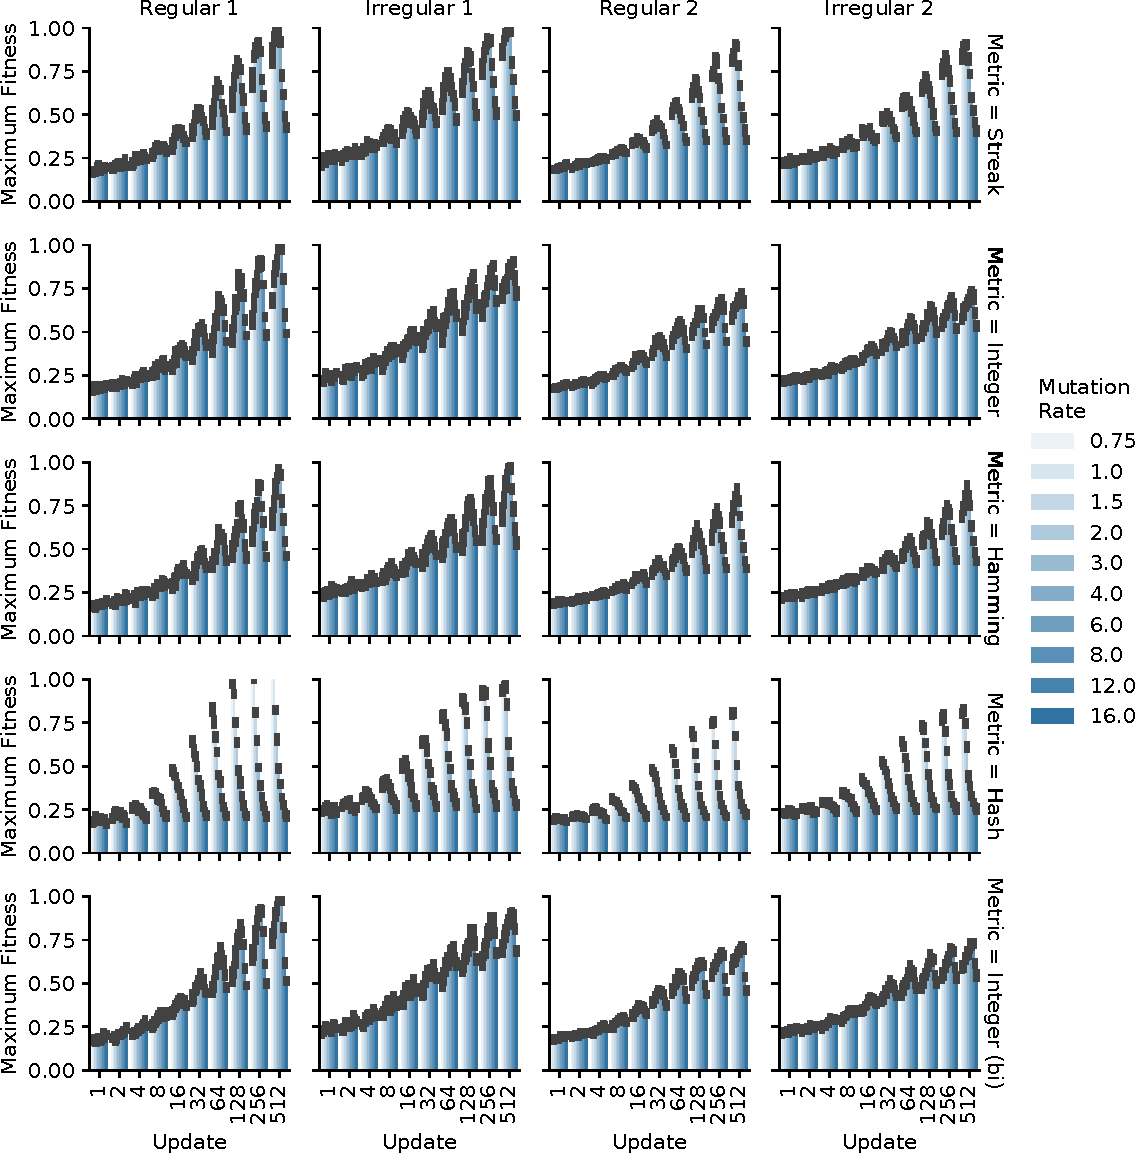
\includegraphics[width=\textwidth]{target_evolve_big/title=fitness_mutation_barplot+_data_hathash_hash=4db1200f9d71a980+_script_fullcat_hash=fe3ddc711c5abfad+ext=}
\caption{
Maximum fitness among replicate runs across a set of per-bit mutation rates.
Error bars represent 95\% confidence intervals.
}
\label{fig:evolve_mutsweep}

\end{center}
\end{figure*}


\section{Hamming Metric} \label{sec:hammingmetric}

Each tag was represented as an ordered, fixed-length bitstring,
\begin{align*}
t = \langle t_0, t_1, t_2, \dots, t_{n-2}, t_{n-1} \rangle
\end{align*}
where
\begin{align*}
\forall i, t_i \in \{0, 1\}.
\end{align*}

This metric is based on the work of \citep{lalejini2019else}, originally after TODO hamming cite(?).

In this metric, we compare tags according to their bitwise hamming distance.
Mathematically speaking for tags $t$ and $u$ we compute the distance according to the metric $M$ as,
\begin{align*}
M(t, u)
= \frac{
  \#\{ i : t_i \neq u_i, i=0, \dots ,n-1\}
}{
  n
}
\end{align*}

This metric is commutative and $n$-dimensional.




\section{Hash Metric} \label{sec:hashmetric}

This metric is original to the our paper and meant to serve as a control.

The an arbitrary, but determinsitic value, uniformly distributed between 0 and 1.

We rely on the \texttt{hash\_combine} function, adapted from BOOST (TODO cite).

for two values \texttt{v1} and \texttt{v2}, \texttt{hash\_combine} is defined as follows
\begin{verbatim}
unsigned int hash_combine(
  unsigned int v1,
  unsigned int v2
) {
  return v1 ^ (
    v2 * 0x9e3779b9
    + (v1 << 6) + (v1 >> 2)
  );
}
\end{verbatim}

We compute the hash value of a tag as follows
\begin{verbatim}
unsigned int h(unsigned char *tag) {
  unsigned int result = tag[0];
  for (int i = 1; i < 4; ++i){
    result = hash_combine(result, t[i]);
  }
  return result;
}
\end{verbatim}
where \texttt{tag} is the tag's bitstring stored as an array of bytes.

To compute the metric $H$ we then call \texttt{hash\_combine} to combine the hash values of the tags $t$ and $u$
\begin{align*}
H(t, u) = \texttt{hash\_combine( h(}t\texttt{), h(}u\texttt{))}
\end{align*}

Note that this is not commutative.




\section{Integer Metric}
\label{sec:integermetric}

Each tag was represented as an ordered, fixed-length bitstring,
\begin{align*}
t = \langle t_0, t_1, t_2, \dots, t_{n-2}, t_{n-1} \rangle
\end{align*}
where
\begin{align*}
\forall i, t_i \in \{0, 1\}.
\end{align*}

This metric is inspired by \citep{spector2011tag}.
They used positive integers between 0 and 100 to name referents.
Queries were provided the referent that had the next-larger value, wrapping around from 100 back to 0.

In this metric, we compare tags according to their value as an unsigned integer according to the following representation $f$,
\begin{align*}
f(t)
= \sum_{i=0}^{n-1} t_i \times 2^i.
\end{align*}

The distance metric $I$ between two length-$n$ tags $t$ and $u$ is
\begin{align*}
I(t, u) =
\begin{cases}
  \frac{2^n - f(t) + f(u)}{2^n}, & \text{if } f(t) > f(u), \\
  \frac{f(t) - f(u)}{2^n},         & \text{else} f(t) \leq f(u).
\end{cases}
\end{align*}

Note that this metric is non-commutative, i.e., it is not necessarily true that $I(t, u) = I(u, t)$.

Note also that this metric is one-dimensional.

A algorithmic advantage of this metric is that it allows for log-time matching.




\subsection{Bidirectional Integer Metric} \label{sec:integerbimetric}

Each tag was represented as an ordered, fixed-length bitstring,
\begin{align*}
t = \langle t_0, t_1, t_2, \dots, t_{n-2}, t_{n-1} \rangle
\end{align*}
where
\begin{align*}
\forall i, t_i \in \{0, 1\}.
\end{align*}

This metric is inspired by \citep{spector2011tag}.
They used positive integers between 0 and 100 to name referents.
Queries were provided the referent that had the next-larger value, wrapping around from 100 back to 0.

In this metric, we compare tags according to their value as an unsigned integer according to the following representation $f$,
\begin{align*}
f(t)
= \sum_{i=0}^{n-1} t_i \times 2^i.
\end{align*}

The distance metric $I$ between two length-$n$ tags $t$ and $u$ is
\begin{align*}
I(t, u) =
\begin{cases}
  \frac{2^n - f(t) + f(u)}{2^n}, & \text{if } f(t) > f(u), \\
  \frac{f(t) - f(u)}{2^n},         & \text{else} f(t) \leq f(u).
\end{cases}
\end{align*}

Note that this metric is non-commutative, i.e., it is not necessarily true that $I(t, u) = I(u, t)$.

Note also that this metric is one-dimensional.




\section{Streak Metric} \label{sec:streakmetric}

Each tag was represented as an ordered, fixed-length bitstring,
\begin{align*}
t = \langle t_0, t_1, t_2, \dots, t_{n-2}, t_{n-1} \rangle
\end{align*}
where
\begin{align*}
\forall i, t_i \in \{0, 1\}.
\end{align*}

This metric was originally proposed by \citep{downing2015intelligence}.
Downing claims that it exhibits
It is computed according to the ratio between the longest contiguously matching substring among two bitsets and the longest contiguously mismatching substring among those two bitsets.
Downing claims that this metric exhibits greater robustness compared to integer and hamming distance metrics using mutational walk experiments but does not demonstrate it in an evolving system.

We define the greatest contiguously-matching length of $n$-long bitstrings $t$ and $u$ as follows,
\begin{align*}
m(t, u) = \max(\{i - j \forall i, j \in 0..n-1 \mid \forall q \in i..j, t_q = u_q \})
\end{align*}

We define the greatest contiguously-mismatching length as follows,
\begin{align*}
n(t, u) = \max(\{i - j \forall i, j \in 0..n-1 \mid \forall q \in i..j, t_q \neq u_q \})
\end{align*}

The streak metric $S'$  with tags $t$ and $u$
\begin{align*}
S'(t, u)
= \frac{ p(n(t,u)) }{p(m(t,u)) + p(n(t,u))}.
\end{align*}
where $p$ approximates the probability of a contiguously-matching substring between

It is worth noting that the formula for computing the probability of a $k$-bit match or mismatch, given by Downing as follows, is actually mathematically flawed.
\begin{align*}
p_k
= \frac{n - k + 1}{2^k}
\end{align*}

The probability of a $0$-bit match according to this formula would be computed as $p_0 = \frac{n - 0 + 1}{2^0} = n + 1$ which is clearly impossible because $p_0 > 1 \forall n > 0$.
The actual can probability be achieved using a lookup table computed using dynamic programming.

However, the formula Downing presented provides a useful approximation to the probability of a $k$ bit match.
For computational efficiency and consistency with the existing literature we use clamp edge cases between 0 and 1 to yield the corrected streak metric $S$.

\begin{align*}
S(t, u) =
\max( \min( S'(t, u), 1), 0)
\end{align*}




\section{Detour Difference}

\begin{figure}
\begin{center}

\begin{minipage}{\linewidth}
\begin{subfigure}[b]{\linewidth}
\begin{minipage}{0.5\textwidth}
\begin{center}
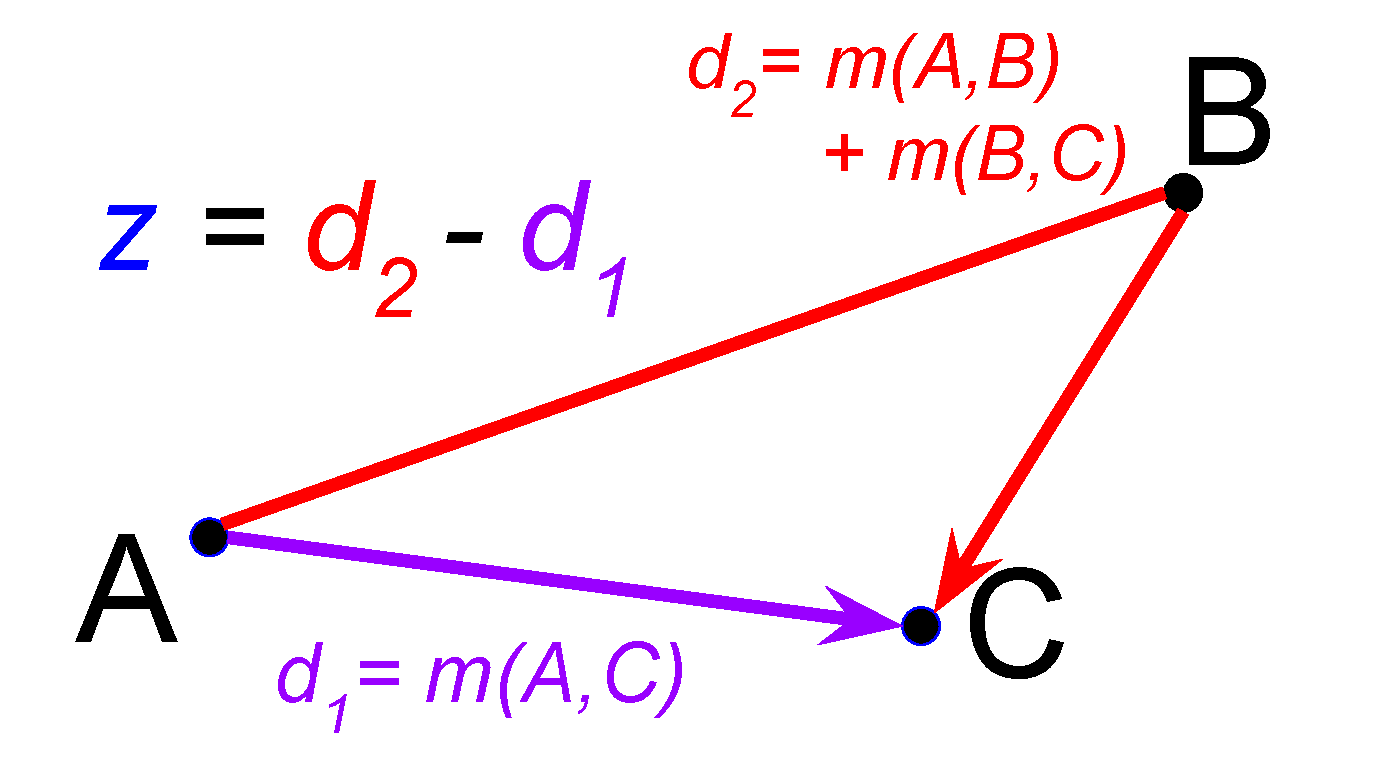
\includegraphics[width=\linewidth,trim=2cm 5cm 2cm 5cm, clip]{detour-difference}
\end{center}
\end{minipage}%
\begin{minipage}{0.5\textwidth}
\caption{
Sampling process used to evaluate detour difference, $z$.
} \label{fig:detour_difference_cartoon}
\end{minipage}
\end{subfigure}
\end{minipage}

\begin{minipage}{\linewidth}
\begin{subfigure}[b]{\linewidth}
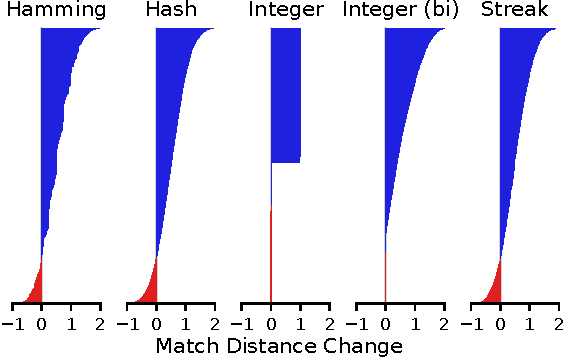
\includegraphics[width=\linewidth]{detour_difference/bitweight=0dot5+seed=1+title=low-triplet-analysis+_data_hathash_hash=6b0749ef97a58721+_script_fullcat_hash=297c4fe09078e17b+ext=}
\caption{
Distributions of detour distance difference for triplets of randomly sampled tags.
Each bar sliver represents an independently sampled observation.
A positive value (colored blue) indicates that total distance increased with the addition of an intermediate stop.
A value of exactly 0 indicates an intermediate stop had no effect on total distance.
A negative value (colored red) indicates violation of the triangle inequality: taking an intermediate stop reduced the total distance travelled.
} \label{fig:detour_difference_distribution}

\end{subfigure}
\end{minipage}

\caption{
Detour difference of tag-matching metrics.
}
\label{fig:detour_difference}

\end{center}
\end{figure}


To get a sense of the regularity, in a looses sense, of each space we uniformly sampled triplets of points $A$, $B$, and $C$.
Then, for each metric $m$ we calculated the statistic $m(A, B) + m(B, C) - m(A, C)$.
If the triangle inequality is respected this statistic should be greater than or equal to zero.
Figure \ref{fig:detour_difference} plots the distribution of this statistic for each metric.
The hamming, hash, and streak metrics show evidence of ``shortcuts'' that violate the triangle inequality.
It should be noted that the raw hamming metric does respect the triangle inequality.





To get a sense of the regularity, in a looses sense, of each space we uniformly sampled triplets of points $A$, $B$, and $C$.
Then, for each metric $m$ we calculated the statistic $m(A, B) + m(B, C) - m(A, C)$.
If the triangle inequality is respected this statistic should be greater than or equal to zero.
Figure \ref{fig:detour_difference} plots the distribution of this statistic for each metric.
The hamming, hash, and streak metrics show evidence of ``shortcuts'' that violate the triangle inequality.
It should be noted that the raw hamming metric does respect the triangle inequality.

\section{Genetic Programming Experiments}
\label{sec:gpsupplement}


\subsection{SignalGP}

SignalGP (Signal-driven Genetic Programs) is a GP representation that enables signal-driven (\textit{i.e.}, event-driven) program execution.
In SignalGP, programs are segmented into modules (functions) that may be automatically triggered by exogenously- or endogenously-generated signals.
Each module in SignalGP associates a tag with a linear sequence of instructions.
SignalGP makes explicit the concept of signals (events), which comprise a tag and, optionally, signal-specific data.
Signals trigger the module with the closest matching tag (according to a given tag-matching scheme), using any signal-associated data as input to the triggered module.
SignalGP can handle many signals simultaneously, processing each in parallel.

The SignalGP instruction set, in addition to including traditional GP operations, allows programs to generate internal signals, broadcast external signals, and otherwise work in a tag-based context.
Instructions contain arguments, including an evolvable tag, that may modify the instruction's effect, often specifying memory locations or fixed values.
Instructions may refer to program modules using tag-based referencing; for example, an instruction may trigger the execution of a program module using the instruction's tag to specify which module to trigger.
SignalGP also supports genetic regulation with promoter and repressor instructions that, when executed, allow programs to adjust how well subsequent signals match with a target function (specified with tag-based referencing).

See \citepinappendix{lalejini2018evolving} for a more detailed description of the SignalGP representation. Additionally, see the GitHub repository for the SignalGP implementation used in this work \citepinappendix{lalejini_2020_3781295}.

\subsection{Changing-signal Task Description}

The changing-signal task requires programs to express a distinct response to each of $K$ environmental signal (each signal has a unique tag).
Programs express a response by executing one of $K$ response instructions.
Successful programs can `hardcode' each response with the appropriate environmental signal, ensuring that each environmental signal's tag best matches the function containing the correct response.
We expect the particular metric used to match tags to influence how well programs adapt to changing-signal task.

During evaluation, we afford programs 64 time steps to express the appropriate response after receiving a signal.
Once a program expresses a response or the allotted time expires, we reset the program's virtual hardware (resetting all executing threads and thread-local memory), and the environment produces the next signal.
Evaluation continues until the program correctly responds to each of the $K$ environmental signals or until the program expresses an incorrect response.
During each evaluation, programs experience environmental signals in a random order; thus, the correct \textit{order} of responses will vary and cannot be hardcoded.

% Experiment overview
For each metric, we evolved 200 replicate populations (each with a unique random number seed) of 500 asexually reproducing programs in an eight-signal environment ($K=8$) for 100 generations.
We identified the most performant tag mutation rate (from a range of possible mutation rates) for each metric to use in our experiment.
These data (and analyses) are available online in the GitHub repository that houses these experiments \citepinappendix{lalejini_2020_3781295}.
We used the following per-bit tag mutation rates for the changing-signal task: 0.01 for the Hamming and Streak metrics, 0.002 for the Hash metric, and 0.02 for the Integer and Bidirectional Integer metrics.
Aside from tag mutation rate, the overall configuration used for each metric was identical.
We limited tag variation in offspring to tag mutation operators (bit flips) by initializing populations with a common ancestor program in which all tags are identical and by disallowing mutations that would insert instructions with random tags.

The full configuration details for the changing-signal task (including a guide to running these experiments on your local machine) can be found in the associated GitHub repository \citepinappendix{lalejini_2020_3781295}.

\subsection{Directional-signal Task Description}

% Task overview
As in the changing-signal task, the directional-signal task requires that programs respond to a sequence of environmental cues; in the directional-signal task, however, the correct response depends on previously experienced signals.
In the directional signal task, there are two possible environmental signals --- a `forward-signal' and a `backward-signal' (each with a distinct tag) ---  and four possible responses.
If a program receives a forward-signal, it should express the next response, and if the program receives, a backward-signal, it should express the previous response.
For example, if response-three is currently required, then a subsequent forward-signal indicates that response-four is required next, while a backward-signal would instead indicate that response-two is required next.
Because the appropriate response to both the backward- and forward-signals change over time, successful programs must regulate which functions these signals trigger (rather than hardcode each response to a particular signal).

% Evaluation overview
We evaluate programs on all possible four-signal sequences of forward- and backward-signals (sixteen total).
For each program, we evaluate each sequence of signals independently, and a program's fitness is equal to its aggregate performance.
Otherwise, evaluation on a single sequence of signals mirrors that of the changing signal task.

% Experiment overview
We used an identical experimental design for the directional-signal task as in the changing-signal task. 
However, we evolved programs for 5000 generations (instead of 100) and re-parameterized each metric's tag mutation rate (these data are available in the associated GitHub repository \citepinappendix{lalejini_2020_3781295}): 
0.001 for the Hamming and Hash metrics, 0.002 for the Integer and Streak metrics, and 0.0001 for the Bidirectional Integer Metric. 

The full configuration details for the directional-signal task (including a guide to running these experiments on your local machine) can be found in the associated GitHub repository \citepinappendix{lalejini_2020_3781295}.

\subsection{Data analysis and Implementation}

The source code for our GP experiments can be found in the following GitHub repository: \citepinappendix{lalejini_2020_3781295}. This repository additionally includes all data analysis and visualization scripts, experiment configuration details, and a guide for running our experiments locally.





\footnotesize
\bibliographystyleinappendix{apalike}
\bibliographyinappendix{bibl} % replace by the name of your .bib file

\end{document}
